\documentclass[]{article}
\usepackage{lmodern}
\usepackage{amssymb,amsmath}
\usepackage{ifxetex,ifluatex}
\usepackage{fixltx2e} % provides \textsubscript
\ifnum 0\ifxetex 1\fi\ifluatex 1\fi=0 % if pdftex
  \usepackage[T1]{fontenc}
  \usepackage[utf8]{inputenc}
\else % if luatex or xelatex
  \ifxetex
    \usepackage{mathspec}
  \else
    \usepackage{fontspec}
  \fi
  \defaultfontfeatures{Ligatures=TeX,Scale=MatchLowercase}
\fi
% use upquote if available, for straight quotes in verbatim environments
\IfFileExists{upquote.sty}{\usepackage{upquote}}{}
% use microtype if available
\IfFileExists{microtype.sty}{%
\usepackage[]{microtype}
\UseMicrotypeSet[protrusion]{basicmath} % disable protrusion for tt fonts
}{}
\PassOptionsToPackage{hyphens}{url} % url is loaded by hyperref
\usepackage[unicode=true]{hyperref}
\hypersetup{
            pdftitle={The specificity of statistical learning},
            pdfauthor={Ansgar Endress},
            pdfkeywords={Keywords},
            pdfborder={0 0 0},
            breaklinks=true}
\urlstyle{same}  % don't use monospace font for urls
\usepackage[margin=1in]{geometry}
\usepackage[sort&compress,numbers]{natbib}
% \bibliographystyle{plainnat}
\bibliographystyle{unsrtnat} 
\usepackage{color}
\usepackage{fancyvrb}
\newcommand{\VerbBar}{|}
\newcommand{\VERB}{\Verb[commandchars=\\\{\}]}
\DefineVerbatimEnvironment{Highlighting}{Verbatim}{commandchars=\\\{\}}
% Add ',fontsize=\small' for more characters per line
\usepackage{framed}
\definecolor{shadecolor}{RGB}{248,248,248}
\newenvironment{Shaded}{\begin{snugshade}}{\end{snugshade}}
\newcommand{\KeywordTok}[1]{\textcolor[rgb]{0.13,0.29,0.53}{\textbf{#1}}}
\newcommand{\DataTypeTok}[1]{\textcolor[rgb]{0.13,0.29,0.53}{#1}}
\newcommand{\DecValTok}[1]{\textcolor[rgb]{0.00,0.00,0.81}{#1}}
\newcommand{\BaseNTok}[1]{\textcolor[rgb]{0.00,0.00,0.81}{#1}}
\newcommand{\FloatTok}[1]{\textcolor[rgb]{0.00,0.00,0.81}{#1}}
\newcommand{\ConstantTok}[1]{\textcolor[rgb]{0.00,0.00,0.00}{#1}}
\newcommand{\CharTok}[1]{\textcolor[rgb]{0.31,0.60,0.02}{#1}}
\newcommand{\SpecialCharTok}[1]{\textcolor[rgb]{0.00,0.00,0.00}{#1}}
\newcommand{\StringTok}[1]{\textcolor[rgb]{0.31,0.60,0.02}{#1}}
\newcommand{\VerbatimStringTok}[1]{\textcolor[rgb]{0.31,0.60,0.02}{#1}}
\newcommand{\SpecialStringTok}[1]{\textcolor[rgb]{0.31,0.60,0.02}{#1}}
\newcommand{\ImportTok}[1]{#1}
\newcommand{\CommentTok}[1]{\textcolor[rgb]{0.56,0.35,0.01}{\textit{#1}}}
\newcommand{\DocumentationTok}[1]{\textcolor[rgb]{0.56,0.35,0.01}{\textbf{\textit{#1}}}}
\newcommand{\AnnotationTok}[1]{\textcolor[rgb]{0.56,0.35,0.01}{\textbf{\textit{#1}}}}
\newcommand{\CommentVarTok}[1]{\textcolor[rgb]{0.56,0.35,0.01}{\textbf{\textit{#1}}}}
\newcommand{\OtherTok}[1]{\textcolor[rgb]{0.56,0.35,0.01}{#1}}
\newcommand{\FunctionTok}[1]{\textcolor[rgb]{0.00,0.00,0.00}{#1}}
\newcommand{\VariableTok}[1]{\textcolor[rgb]{0.00,0.00,0.00}{#1}}
\newcommand{\ControlFlowTok}[1]{\textcolor[rgb]{0.13,0.29,0.53}{\textbf{#1}}}
\newcommand{\OperatorTok}[1]{\textcolor[rgb]{0.81,0.36,0.00}{\textbf{#1}}}
\newcommand{\BuiltInTok}[1]{#1}
\newcommand{\ExtensionTok}[1]{#1}
\newcommand{\PreprocessorTok}[1]{\textcolor[rgb]{0.56,0.35,0.01}{\textit{#1}}}
\newcommand{\AttributeTok}[1]{\textcolor[rgb]{0.77,0.63,0.00}{#1}}
\newcommand{\RegionMarkerTok}[1]{#1}
\newcommand{\InformationTok}[1]{\textcolor[rgb]{0.56,0.35,0.01}{\textbf{\textit{#1}}}}
\newcommand{\WarningTok}[1]{\textcolor[rgb]{0.56,0.35,0.01}{\textbf{\textit{#1}}}}
\newcommand{\AlertTok}[1]{\textcolor[rgb]{0.94,0.16,0.16}{#1}}
\newcommand{\ErrorTok}[1]{\textcolor[rgb]{0.64,0.00,0.00}{\textbf{#1}}}
\newcommand{\NormalTok}[1]{#1}
\usepackage{graphicx,grffile}
\makeatletter
\def\maxwidth{\ifdim\Gin@nat@width>\linewidth\linewidth\else\Gin@nat@width\fi}
\def\maxheight{\ifdim\Gin@nat@height>\textheight\textheight\else\Gin@nat@height\fi}
\makeatother
% Scale images if necessary, so that they will not overflow the page
% margins by default, and it is still possible to overwrite the defaults
% using explicit options in \includegraphics[width, height, ...]{}
\setkeys{Gin}{width=\maxwidth,height=\maxheight,keepaspectratio}
\usepackage[normalem]{ulem}
% avoid problems with \sout in headers with hyperref:
\pdfstringdefDisableCommands{\renewcommand{\sout}{}}
\IfFileExists{parskip.sty}{%
\usepackage{parskip}
}{% else
\setlength{\parindent}{0pt}
\setlength{\parskip}{6pt plus 2pt minus 1pt}
}
\setlength{\emergencystretch}{3em}  % prevent overfull lines
\providecommand{\tightlist}{%
  \setlength{\itemsep}{0pt}\setlength{\parskip}{0pt}}
\setcounter{secnumdepth}{5}
% Redefines (sub)paragraphs to behave more like sections
\ifx\paragraph\undefined\else
\let\oldparagraph\paragraph
\renewcommand{\paragraph}[1]{\oldparagraph{#1}\mbox{}}
\fi
\ifx\subparagraph\undefined\else
\let\oldsubparagraph\subparagraph
\renewcommand{\subparagraph}[1]{\oldsubparagraph{#1}\mbox{}}
\fi

% set default figure placement to htbp
\makeatletter
\def\fps@figure{htbp}
\makeatother

\newcommand{\citeeg}[1]{\cite<e.g.,>[]{#1}}
\newcommand{\cites}[1]{\citeauthor{#1}'s \citeyear{#1}}
\newcommand{\T}{{\em t\/}}
\newcommand{\F}{{\em F\/}}
\newcommand{\Z}{{\em Z\/}}
\newcommand{\p}{{\em p\/}}
\newcommand{\M}{{\em M\/}}
\newcommand{\SD}{{\em SD\/}}
\newcommand{\SE}{{\em SE\/}}
\newcommand{\D}{Cohen's {\em d\/}}
\newcommand{\CI}{$CI_{.95}$}
\newcommand{\et}{$\eta^2$}
\newcommand{\etp}{$\eta_p^2$}
\renewcommand{\U}{{\em U\/}}
\newcommand{\W}{{\em W\/}}
\newcommand{\I}{\mathcal{I}}
\newcommand{\decay}{\mathcal{D}}

\newcommand{\N}{{\mathbf N}}                   %Non-negative integers
\newcommand{\R}{{\mathbf R}}                   %Reals


\newcommand{\colorize}[1]{{\color{red}{#1}}}

% Insert sub-figures without sub-captions but labeling the sub-figures
\newcommand{\includesubgraphics}[2]{
  \begin{subfigure}[a][][t]{.9\textwidth}
    
    {\Large \bf #1 \vspace{-\baselineskip}} 
    
    \hspace{1em}\includegraphics[width=0.9\linewidth]{#2} 
  \end{subfigure}   
}

\renewcommand{\appendixname}{Supplementary Online Materials}

\newcommand{\myappendix}{%
  % For supplementary material, number appendices arabically
  \clearpage
   \setcounter{section}{0}
  \renewcommand{\thesection}{SOM\arabic{section}}
  % Make sure that subsections are correctly numbered
  \renewcommand{\thesubsection}{\thesection.\arabic{subsection}}

  \setcounter{figure}{0}
  \setcounter{table}{0} %
  \renewcommand{\thefigure}{S\arabic{figure}}
  \renewcommand{\thetable}{S\arabic{table}}

  \clearpage
  {\noindent {\LARGE {\bf Supplementary Online Materials}}}
}

\newcommand{\appsectionFirst}[1]{
  % \section for appendix: Reset counters for subsection and figures
  % Doesn't clear page before section
  % \clearpage
  \section{#1}
  \setcounter{subsection}{0}%
}

\newcommand{\appsection}[1]{
  % \section for appendix: Reset counters for subsection and figures
  % Clears page before section
  \clearpage
  \section{#1}
  \setcounter{subsection}{0}%
}


\usepackage{booktabs}
\usepackage{longtable}
\usepackage{array}
\usepackage{multirow}
\usepackage{wrapfig}
\usepackage{float}
\usepackage{colortbl}
\usepackage{pdflscape}
\usepackage{tabu}
\usepackage{threeparttable}
\usepackage{threeparttablex}
\usepackage[normalem]{ulem}
\usepackage{makecell}
\usepackage{xcolor}

\title{The specificity of statistical learning}
\author{Ansgar Endress}
\date{}

\begin{document}
\maketitle
\begin{abstract}
Statistical Learning is ubiquitous across domains and species, and might be critical for the earliest stages of language acquisition, for example to identify and memorize words from fluent speech. However, other forms of associative learning are remarkably tuned to the ecological learning situations, and often dissociable from declarative memory. Here, we show that Statistical Learning selectively operates in certain learning situations, and is dissociable from (declarative) memory mechanisms that allow learners to place word-like items in memory. Statistical Learning predominantly operates in continuous speech sequences similar to those used in prior experiments, but not in discrete chunk sequences, even though the latter are likely encountered during language acquisition (due to the prosodic organization of language). Conversely, when exposed to continuous sequences in a memory recall experiment, participants are sensitive to probable syllable transitions, but, to the extent that they remember any items at all, they tend to initiate their productions with random syllables rather than with word onsets, leading to greater recall of \emph{low-}probablility chunks. In contrast, familiarization with discrete sequences produces reliable memories of actual, high-probability forms. This dissociation between Statistical Learning and memory suggests that Statistical Learning might have a specialized role when distributional information can be accumulated (e.g., for predictive processing), and that it is separable from the (declarative) memory mechanisms needed to acquire words.
\end{abstract}


\section{PNAS FORMAT}\label{pnas-format}

Research reports describe the results of original research of exceptional importance. The preferred length of these articles is 6 pages, but PNAS allows articles up to a maximum of 12 pages. A standard 6-page article is approximately 4,000 words, 50 references, and 4 medium-size graphical elements (i.e., figures and tables).

Templates are available at \url{https://www.pnas.org/authors/submitting-your-manuscript\#manuscript-formatting-guidelines}

A manuscript file (in any format) including the following: * Title page (title, author list, classification, keywords) * Abstract (\textless{} 250 w) * Significance statement (\textless{} 120 w) * Main text - Introduction - Results - Discussion - Materials and methods (describe procedures in sufficient detail so that the work can be repeated) * Acknowledgments and funding sources * References

\begin{itemize}
\tightlist
\item
  Figures or tables with appropriate legends (may be uploaded
  separately)
\item
  SI files (may be uploaded separately)
\item
  Contact and competing interest information for all authors.
\item
  Data sharing plans (for all data, documentation, and code used in
  analysis).
\item
  Funding information and whether an open access license has been
  selected.
\item
A list of appropriate Editorial Board, NAS members, and qualified reviewers (minimum of three each) who are experts in the * paper's scientific area. A brief justification for suggested reviewers is welcome, particularly for interdisciplinary papers.
\end{itemize}

\section{Significance statement (\textless{}
120w)}\label{significance-statement-120w}

\section{Introduction}\label{introduction}

% Unused references
%% General Statistics
% Conway2005a
%% Preferential associations
% Seligman1970
%% TPs as predictive processing/associative learning
% Goujon2015
%% Dissociations between declarative and implicit memory
% Cohen1980
%% Predictive processing
% Bar2009
%% Infant sensitivity to prosody
%Hirsh-Pasek1987; Christophe1994; Gout2004
%% Known words and segmentation
%Shi2008; Weijer1999


Associative learning is remarkably widespread across species and domains \citep{Aslin1998,Chen2015,Fiser2002,Hauser2001,Saffran-Science,Toro2005-backward,Turk-Browne-reversal}, and might support a wide range of computations, especially during language acquisition \citep{Aslin2012, Seidenberg2002}.

However, associative learning is also remarkably modular \citep{Endress-duplications}. Humans have independent associative learning abilities in superficially similar domains, including associations of objects with landmarks vs.~boundaries \citep{Doeller2008}, associations among social vs.~non-social objects \citep{Tompson2019} and associations among consonants vs.~vowels \citep{Bonatti2005,Toro2008}. Likewise, preferential associations abound. For example, rats readily associate tastes with sickness and external stimuli with pain, but cannot associate taste with pain or external stimuli with sickness \citep{Garcia1974}. Such patterns of associations reflect the likely ecological sources of sickness vs.~pain (i.e., food vs.~external events), and can evolve in just 40 generations in fruit flies \citep{Dunlap2014}.

Critically, some associations can be detrimental, and are thus blocked. For example, taste-sickness associations (but not other associations) are blocked in a suckling context for rat pups with no exposure to solid food \citep{Martin1979, Alberts1984}, presumably because avoidance of the \emph{only} food source is costly; in contrast, minimal exposure to solid food re-establishes taste-sickness associations \citep{Gubernick1984}.

While such results suggest that, over evolutionary times, the availability of associative learning can be modified for specific stimulus classes, it is less clear if associative learning is specialized for specific computational functions - or essentially a side effect of local neural processing \citep[a ``spandrel'' in biological terms;][]{Gould1979} that is sometimes adaptive, sometimes neutral and sometimes detrimental. Here, we address this issue in a domain where the importance of associative learning has long been recognized: learning words from fluent speech. We suggest that associative learning is critical for predicting speech material and operates predominantly under conditions where prediction is possible. However, we also suggest that separate mechanisms are required to form (declarative) memories of the words learners need to acquire.

Speech is thought to be a continuous signal, and before learners can commit any words to memory, they need to learn where words start and where they end. They might rely on Transitional Probabilities (TPs) among items, that is, the conditional probability of a syllable \(\sigma_{i+1}\) given a preceding syllable \(\sigma_{i}\), \(P(\sigma_{i}\sigma_{i+1})/P(\sigma_{i})\). Relatively predictable transitions are likely located inside words, while unpredictable ones straddle word boundaries. Early on, Shannon \citep{Shannon1951} showed that human adults are sensitive to such distributional information. Subsequent work demonstrated that infants and non-human animals share this ability \citep{Aslin1998, Chen2015, Fiser2002, Hauser2001, Saffran-Science, Toro2005-backward}, and that it might reflect simple associative mechanisms such as Hebbian learning \citep{Endress-TP-Model}.


Associative knowledge might be critical for predictive processing \citep{Sherman2020, Turk-Browne2010}, an ability that is critical for both language \citep{Levy2008, Trueswell1999} and other cognitive processes \citep{Clark2013, Friston2010, Keller2018}. However, such knowledge does not imply that learners store words in (declarative) long-term memory. In fact, observers prefer high-TP items to low-TP items even if they have never encountered the items and thus could now have memorized them (because the items are played backwards; \citealp{Turk-Browne-reversal,Jones2007}, and sometimes even prefer high-TP items they have \emph{never} encountered to low-TP items they have heard or seen \citep{Endress-Phantoms-Vision}. Such results suggest that associative learning and memory for specific chunks may be dissociable (see also \citealp{Knowlton1996a, Poldrack2001, Squire1992} and Discussion), a view that is reinforced by the suggestion that representations created by associative learning differ from those used for linguistic stimuli \citep{Endress-Phantoms-Vision, Fischer-Baum2011}. 

Here, we explore the computational function of associative learning, focusing on the conditions under which it operates and its relation to memory processes. To explore its operating conditions, we note that speech does not come as a continuous signal but rather as a sequence of smaller units due to its prosodic organization \citep{Cutler1997, Nespor1986, Shattuck-Hufnagel1996}. This prosodic organization is perceived in unfamiliar languages \citep{Brentari2011, Endress-cross-seg, Fenlon2008, Pilon1981} and even by newborns \citep{Christophe2001}. This prosodic information might affect the usefulness of statistical learning, because associative learning operates primarily \emph{within} rather than across major prosodic boundaries \citep{Shukla2007}. As result, the learner's segmentation task is not so much to integrate distributional information over long stretches of continuous speech, but rather to decide whether the correct grouping in prosodic groups such as ``\emph{thebaby}'' is ``\emph{theba + by}'' or ``\emph{the + baby}'' (though prosodic groups are often longer than just three syllables; \citealt{Nespor1986}).

In Experiment 1, we thus ask whether associative learning operates in such smaller chunks, or only in longer stretches of continuous speech. In Experiment 2, we seek to elucidate the function of associative learning, asking (adult) participants to recall what they remember after being exposed to the speech stream from Saffran et al.'s \citep{Saffran-Science} classic experiment, again with a continuous speech stream or a sequence of pre-segmented syllable sequences.

\clearpage


\section{Results}\label{results}

%\subsection{\texorpdfstring{Recognition experiments (Results with the \emph{us3} voice; the \emph{en1} results are in the SI)}{Recognition experiments (Results with the us3 voice; the en1 results are in the SI)}}\label{recognition-experiments-results-with-the-us3-voice-the-en1-results-are-in-the-si}

In Experiment 1, participants listened to a speech sequence of tri-syllabic words. The words were either \emph{pre-segmented} (i.e., with a silence after each word) or continuously concatenated. For half of the participants, both the TPs and the chunk frequency was higher between the the first two syllables of the word than between the last two syllables. An associative learner should thus split a triplet like \emph{ABC} into an initial \emph{AB} chunk followed by a singleton \emph{C} syllable (hereafter \emph{AB+C} pattern). For the remaining participants, both the TPs and the chunk frequency favored an \emph{A+BC} pattern. Following this familiarization, they heard pairs of \emph{AB} and \emph{BC} items, and had to indicate which item was more like the familiarization items.


%\subsubsection{Can people recover words from pre-segmented prosodic units?}\label{can-people-recover-words-from-pre-segmented-prosodic-units}

When the familiarization stream was pre-segmented, participants failed to split smaller utterances into their underlying components. As shown in Figure \ref{fig:stats-london-stats.3x.us.segm.cont.plot}, the average performance did not differ significantly from the chance level of 50\%, (\M~= 51.67, \SD~= 15.17), \(V\) = 216, \(p\) = 0.307. Likelihood ratio analysis favored the null hypothesis by a factor of 4.57 after correction with the Bayesian Information Criterion. As shown in Table \ref{tab:stats-london-stats.us.lang.glmm.print}, performance did not depend on the language condition. As shown in SI~\ref{app:exp_en1_segm}, this failure was replicated using a second voice (\emph{en1}, British English male). The failure to use statistical learning to split pre-segmented units was conceptually replicated in a pilot experiment with Spanish/Catalan speakers using chunk frequency and backwards TPs as the primary cues (SI \ref{app:pilot_bcn}).

%\subsubsection{Can people recover words from a continuous stream? (1)}\label{can-people-recover-words-from-a-continuous-stream-1}

In contrast to the common finding that humans and other animals are sensitive to TPs, our participants failed to use TPs to split pre-segmented utterances into their underlying units. We thus asked if, in line with previous research, they can track TPs units are embedded into a \emph{continuous} speech stream. That is, participants listened to the very same speech stream as in the pre-segmented condition, except that the stream was continuous.

As shown in Figure \ref{fig:stats-london-stats.3x.us.segm.cont.plot}, the average performance differed significantly from the chance level of 50\%, (\M~= 58.51, \SD~= 16.21), \D~= 0.52, \CI~= 52.66, 64.35, \(V\) = 306.5, \(p\) = 0.0185. As shown in Table \ref{tab:stats-london-stats.us.lang.glmm.print}, performance did not depend on the language condition, and was marginally better than in the pre-segmented condition (\p~= .08).

%\subsubsection{Can people recover words from a continuous stream? (2) (Replication)}\label{can-people-recover-words-from-a-continuous-stream-2-replication}

We replicated the successful tracking of statistical information using a new sample of participants. As shown in Figure \ref{fig:stats-london-stats.3x.us.segm.cont.plot}, the average performance differed significantly from the chance level of 50\%, (\M~= 62.78, \SD~= 21.35), \D~= 0.6, \CI~= 54.81, 70.75, \(V\) = 320, \(p\) = 0.00778. As shown in Table \ref{tab:stats-london-stats.us.lang.glmm.print}, performance did not depend on the language condition, and was significantly better than in the pre-segmented condition (\p~= .013).

(As shown in SI \ref{app:exp_en1_cont}, this result could not be replicated using a different voice (\emph{en1}, male British English); participants seemed to prefer specific items, presumably because the synthesizer produced click-like sounds for some stops and fricatives that likely affected syllable grouping.)

Taken together, these results thus suggest that associative learning predominantly operates in continuous sequences, but less so in pre-segmented sequences. Such a result is compatible with the view that associative learning is important for predictive processing, given that continuous sequences are more conducive for prediction. In contrast, it raises doubts as to whether participants can use associative learning to memorize words, given that they do not seem to be able to do so in pre-segmented streams.

\begin{figure}

{\centering 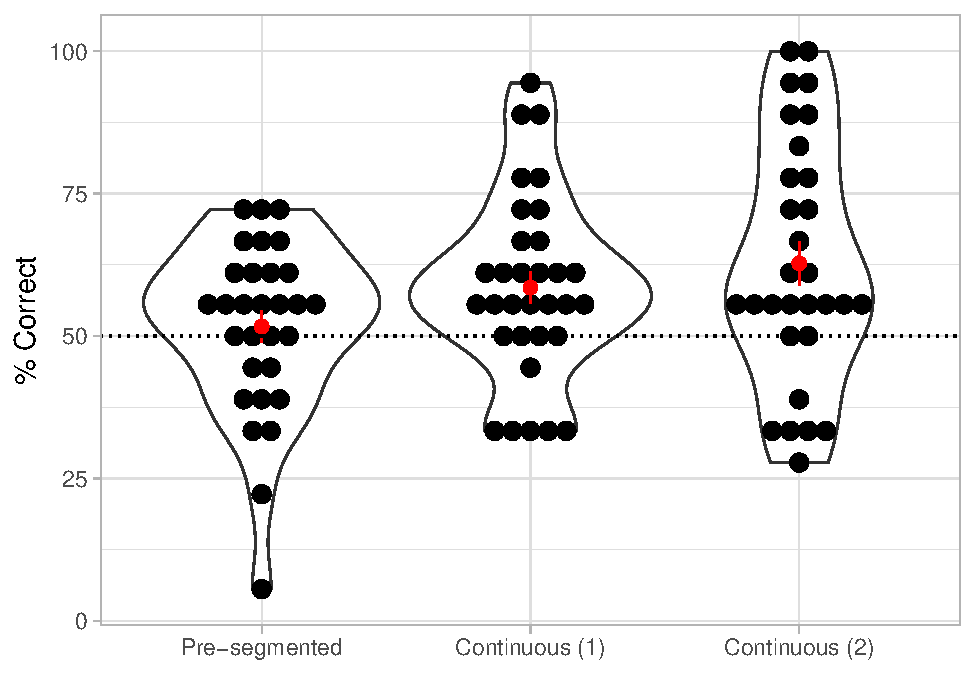
\includegraphics[width=0.8\linewidth]{segmentation_recall_combined_files/figure-latex/stats-london-stats.3x.us.segm.cont.plot-1} 

}

\caption{Results of Experiment 1. Each dot represents a participant. The central red dot is the sample mean; error bars represent standard errors from the mean. The results show the percentage of correct choices in the recognition test after familiarization with (left) a pre-segmented familiarization stream or (middle, right) a continuous familiarization stream. The two continuous conditions are replictions of one another.}\label{fig:stats-london-stats.3x.us.segm.cont.plot}
\end{figure}



\clearpage

%\subsection{Recall experiment}\label{recall-experiment-1}

In Experiment 2, we explored the computational function of associative learning, and asked if participants would remember the items that occurred in a speech stream. Adult participants listened to the artificial languages \citet{Saffran-Science} used with 8-months-olds, except that we doubled the exposure. The languages comprised four words, with a TP of 1.0 within words and 0.33 across word boundaries. The words were presented in a continuous stream or as a pre-segmented word sequence. We ran both a lab-based and an online version of this experiment. Lab-based participants just listened to the speech stream, while online participants watched an astronomical video at the same time.

Following a retention interval, participants had to repeat back the words they remembered from the speech stream. Lab-based participants responded vocally, while online participants typed their answer into a comment field. Finally, participant completed a recognition test during which we pitted words against part-words. Part-words are tri-syllabic items that straddle a word-boundary. For example, if \emph{ABC} and \emph{DEF} are two consecutive words, \emph{BCD} and \emph{CDE} are the corresponding part-words. If participants reliably choose words over part-words, they track TPs.

In the analyses below, we removed single syllable responses (and participants who did not produce any other other items). We also removed participants who did not perform at least 50\% during the final recognition test.

%\subsubsection{General measures}\label{general-measures}
%\subsubsection{TP-based analyses}\label{tp-based-analyses}

As shown in Table \ref{tab:recall-all-results-print} and Figures \ref{fig:recall-general-measures-tp-plot}a and b, participants produced about 4 items. Neither the number of items produced nor their lengths differed across the segmentation conditions. Critically, and as shown in Table \ref{tab:recall-all-results-print} and Figures \ref{fig:recall-general-measures-tp-plot}c and d, forward and backward TPs in the participants' responses were significantly greater than the chance level of \(.083\) in both segmentation conditions. These TPs likely underestimate the participants' performance, as we included responses with unattested syllables that might reflect misperceptions; after removing such responses, TPs in the participants' responses were about twice as large. Participants were thus clearly sensitive to the TPs in the speech stream. (TPs were somewhat higher in the pre-segmented condition. This finding does not contradict the results from the Experiment 1 above; after all, if participants faithfully recall familiarization items, the resulting TPs will be high as well.)

%\subsubsection{Word vs.~part-word analysis}\label{word-vs.part-word-analysis}

The traditional analysis of word segmentation experiments relies on the contrast between words and part-words. As mentioned above, part-words are tri-syllabic items that straddle a word-boundary. We thus calculated the proportion of words among words and part-words or concatenations of words and part-words. If participants faithfully produce trisyllabic sequences from the stream, they can start the sequences on the first, second or third syllable of a word, but only the first possibility yields words rather than part-words. As a result, if participants initiate their productions with a random syllable, a third of their productions should be words.

As shown in Table \ref{tab:recall-all-results-print} and in Figure \ref{fig:recall-w-pw-chunks-positions-plot}a, the proportion of words among words and part-words was close to 100\% in the pre-segmented condition, but did not differ from the chancel level of 1/3 in the continuous condition. Likelihood ratio analysis suggests that, in the continuous condition, participants were 3.5 more likely to perform at the chance level of 33\% (2.6 for the lab-based experiments) than to perform at a level different from chance. These results thus suggest that participants in the continuous condition initiate their productions at random positions in the stream, and that they did not remember any word forms.

However, inspection of Figure \ref{fig:recall-w-pw-chunks-positions-plot}a shows that the distribution after continuous sequences is bimodal, with some participants producing only words, and others producing only part-words. Assuming that the number of participants producing words vs.~part-words follows a binomial distribution, we can thus calculate the likelihood ratio of a model where learners identify word boundaries (and should thus produce words with probability 1), and a model where they track TPs and initiate productions at random positions (and should produce words with a probability of 1/3). As shown in SI \ref{app:likelihood}, the likelihood ratio in favor of the first model is \(3^{N_W}\) if participants produce no part-words (i.e., after a pre-segmented familiarization), where \(N_W\) is the number of participants producing words; otherwise, the likelihood ratio in favor of the second model is infinity. These results thus suggest that, despite their ability to track TPs, participants initiate productions at random positions in the sequence, and thus do not remember statistically defined words.

However, as shown in Figure \ref{fig:recall-words-part-words-raw-plot}, these results might be misleading because, in the continuous condition, many participants produce neither words \emph{nor} part-words. In fact, on average, they produce only .4 words and part-words combined, respectively. (In the pre-segmented condition, most participants produce at least one word, with an average of 1.26.) Given that participants produce few tri-syllabic items, we thus focus on shorter chunks.

%\subsubsection{TP-based chunks analysis}\label{tp-based-chunks-analysis}

We first focus on bisyllabic chunks. They are either high-TP chunks that are part of a word, or low-TP chunks that straddle a word boundary. For example, with two consecutive words \emph{ABC} and \emph{DEF}, the high-TP chunks are \emph{AB}, \emph{BC}, \ldots{}, while the low-TP chunk is \emph{CD}. As a result, two-syllable items have a 66\% probability of being a high-TP chunk. As shown in Figure \ref{fig:recall-w-pw-chunks-positions-plot}b, the proportion of high-TP among chunks high- and low-TP chunks exceeded chance in the pre-segmented condition, but not in the continuous condition. In the continuous condition, the likelihood ratio in favor of the null hypothesis is 0.652 (1.892 for the lab-based experiments). These results are thus consistent with the possibility that, in the continuous condition, participants do track TPs, but initiate their productions at random positions.

%\subsubsection{Positional analyses}\label{positional-analyses}

Finally, we analyze the productions in terms of correct initial final syllables. As there are four words with one correct initial and final syllable each, and 12 syllables in total, 4/12 of the productions should have ``correct'' initial syllables, and 4/12 should have correct final syllables.

As shown in Table \ref{tab:recall-all-results-print} and Figure \ref{fig:recall-w-pw-chunks-positions-plot}c and d, participants produced items with correct initial or final syllables at greater than chance level only in the segmented condition, but not the continuous condition. In the continuous condition, the likelihood ratio in favor of the null hypothesis was 0.785 for initial syllables (3.606 for the lab-based experiment) and 4.061 for final syllables (2.139 for the lab-based experiment).

\begin{table}

\caption{\label{tab:recall-all-results-print}Various analyses pertaining to the productions as well as test against their chances levels.}
\centering
\resizebox{\linewidth}{!}{
\begin{tabular}[t]{l>{\raggedright\arraybackslash}p{20em}>{\raggedright\arraybackslash}p{20em}>{\raggedleft\arraybackslash}p{15em}}
\toprule
 & Continuous & Segmented & \p (Continuous vs. Segmented)\\
\midrule
\addlinespace[0.3em]
\multicolumn{4}{l}{\textbf{Recognition accuracy}}\\
\hspace{1em}lab-based & \M = 0.615, \SE = 0.048, \p = 0.048 & \M = 0.923, \SE = 0.046, \p = 0.0012 & 0.012\\
\hspace{1em}online & \M = 0.628, \SE = 0.0318, \p = 7.84e-05 & \M = 0.911, \SE = 0.0193, \p = 7.08e-15 & < 0.001\\
\addlinespace[0.3em]
\multicolumn{4}{l}{\textbf{Number of items}}\\
\hspace{1em}lab-based & \M = 4.23, \SE = 0.756, \p = 0.0016 & \M = 4.23, \SE = 0.818, \p = 0.00152 & 0.812\\
\hspace{1em}online & \M = 4.03, \SE = 0.292, \p = 3.17e-14 & \M = 3.25, \SE = 0.202, \p = 2.74e-14 & 0.099\\
\addlinespace[0.3em]
\multicolumn{4}{l}{\textbf{Number of syllables/item}}\\
\hspace{1em}lab-based & \M = 3.79, \SE = 0.421, \p = 0.0016 & \M = 2.97, \SE = 0.0246, \p = 0.0007 & 0.026\\
\hspace{1em}online & \M = 2.65, \SE = 0.0869, \p = 2.29e-14 & \M = 2.93, \SE = 0.0364, \p = 1.04e-15 & < 0.001\\
\addlinespace[0.3em]
\multicolumn{4}{l}{\textbf{Proportion of words among words and part-words (or concatenations thereof)}}\\
\hspace{1em}lab-based & \M = 0.321, \SE = 0.153, 0.798 (vs. 1/3) & \M = 1, \SE = 0, \p = 0.0006 (vs. 1/3) & 0.034\\
\hspace{1em}online & \M = 0.417, \SE = 0.105, \p = 0.189 (vs. 1/3) & \M = 1, \SE = 0, \p = 2.08e-13 (vs. 1/3) & < 0.001\\
\addlinespace[0.3em]
\multicolumn{4}{l}{\textbf{Forward TPs}}\\
\hspace{1em}lab-based & \M = 0.301, \SE = 0.0702, \p = 0.0107 & \M = 0.634, \SE = 0.092, \p = 0.00159 & 0.006\\
\hspace{1em}online & \M = 0.397, \SE = 0.0316, \p = 6.26e-12 & \M = 0.583, \SE = 0.04, \p = 3.82e-13 & 0.001\\
\addlinespace[0.3em]
\multicolumn{4}{l}{\textbf{Backward TPs}}\\
\hspace{1em}lab-based & \M = 0.301, \SE = 0.0702, \p = 0.0107 & \M = 0.634, \SE = 0.092, \p = 0.00159 & 0.006\\
\hspace{1em}online & \M = 0.397, \SE = 0.0316, \p = 6.26e-12 & \M = 0.583, \SE = 0.04, \p = 3.82e-13 & 0.001\\
\addlinespace[0.3em]
\multicolumn{4}{l}{\textbf{Proportion of High-TP chunks among High- and Low-TP chunks}}\\
\hspace{1em}lab-based & \M = 0.75, \SE = 0.289, \p = 0.85 (vs. 2/3) & \M = 1, \SE = 0, \p = 0.0006 (vs. 2/3) & 1.000\\
\hspace{1em}online & \M = 0.767, \SE = 0.0459, \p =  0.00154 (vs. 2/3) & \M = 0.97, \SE = 0.0187, \p = 6.75e-13 (vs. 2/3) & < 0.001\\
\addlinespace[0.3em]
\multicolumn{4}{l}{\textbf{Proportion of items with correct initial syllables}}\\
\hspace{1em}lab-based & \M = 0.333, \SE = 0.105, \p = 0.856 & \M = 0.809, \SE = 0.0694, \p = 0.00186 & 0.016\\
\hspace{1em}online & \M = 0.419, \SE = 0.0392, \p = 0.0864 & \M = 0.738, \SE = 0.0387, \p = 1.58e-11 & 0.000\\
\addlinespace[0.3em]
\multicolumn{4}{l}{\textbf{Proportion of items with correct final syllables}}\\
\hspace{1em}lab-based & \M = 0.456, \SE = 0.125, \p = 0.5 & \M = 0.818, \SE = 0.0829, \p = 0.00222 & 0.025\\
\hspace{1em}online & \M = 0.386, \SE = 0.043, \p = 0.456 & \M = 0.7, \SE = 0.0437, \p = 4.14e-10 & 0.000\\
\bottomrule
\end{tabular}}
\end{table}

\begin{figure}

{\centering 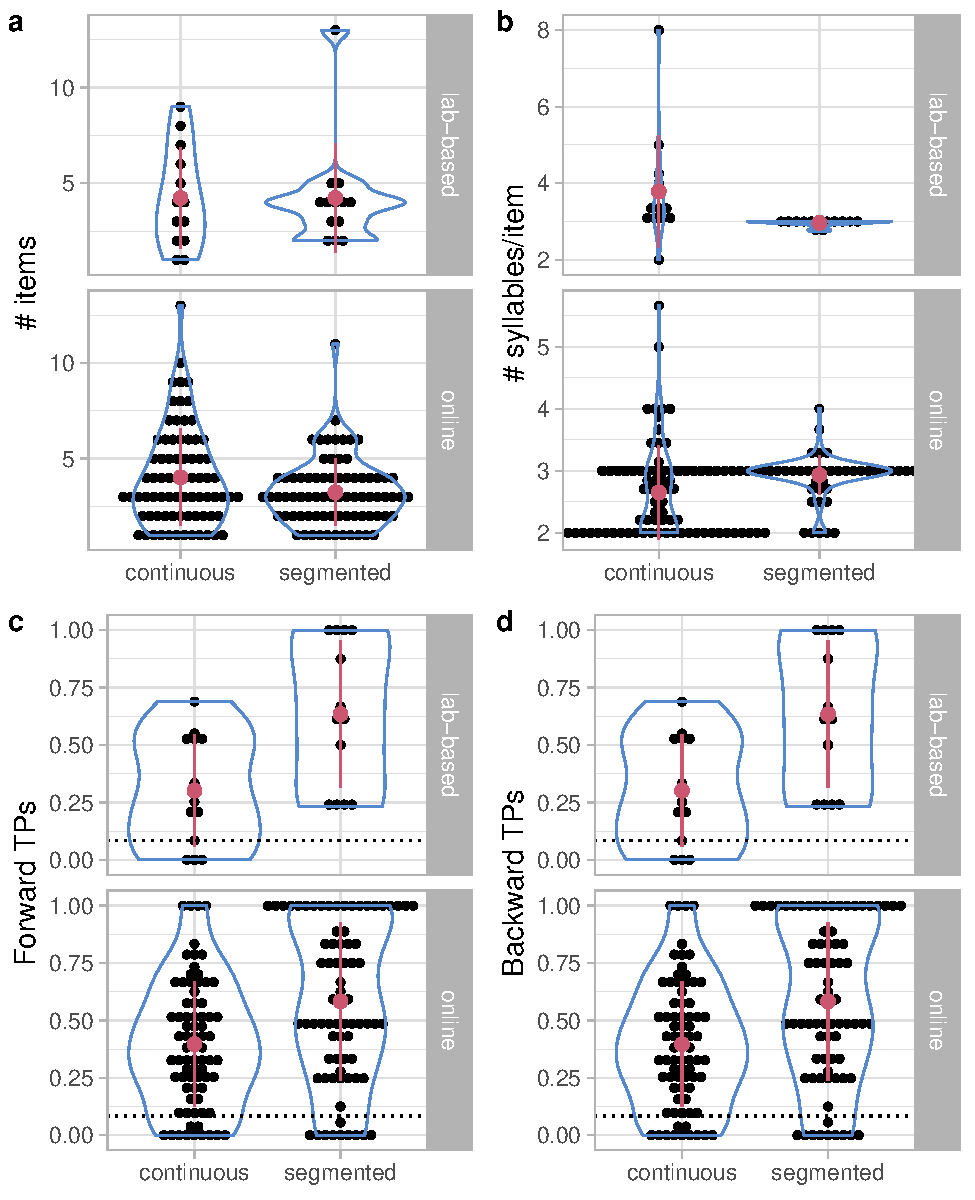
\includegraphics[width=0.8\linewidth]{segmentation_recall_combined_files/figure-latex/recall-general-measures-tp-plot-1} 

}

\caption{Number of items produced, number of syllables per item and forward and backward TPs. The dotted line represents the chance level for a randomly ordered syllable sequence.}\label{fig:recall-general-measures-tp-plot}
\end{figure}

\begin{figure}

{\centering 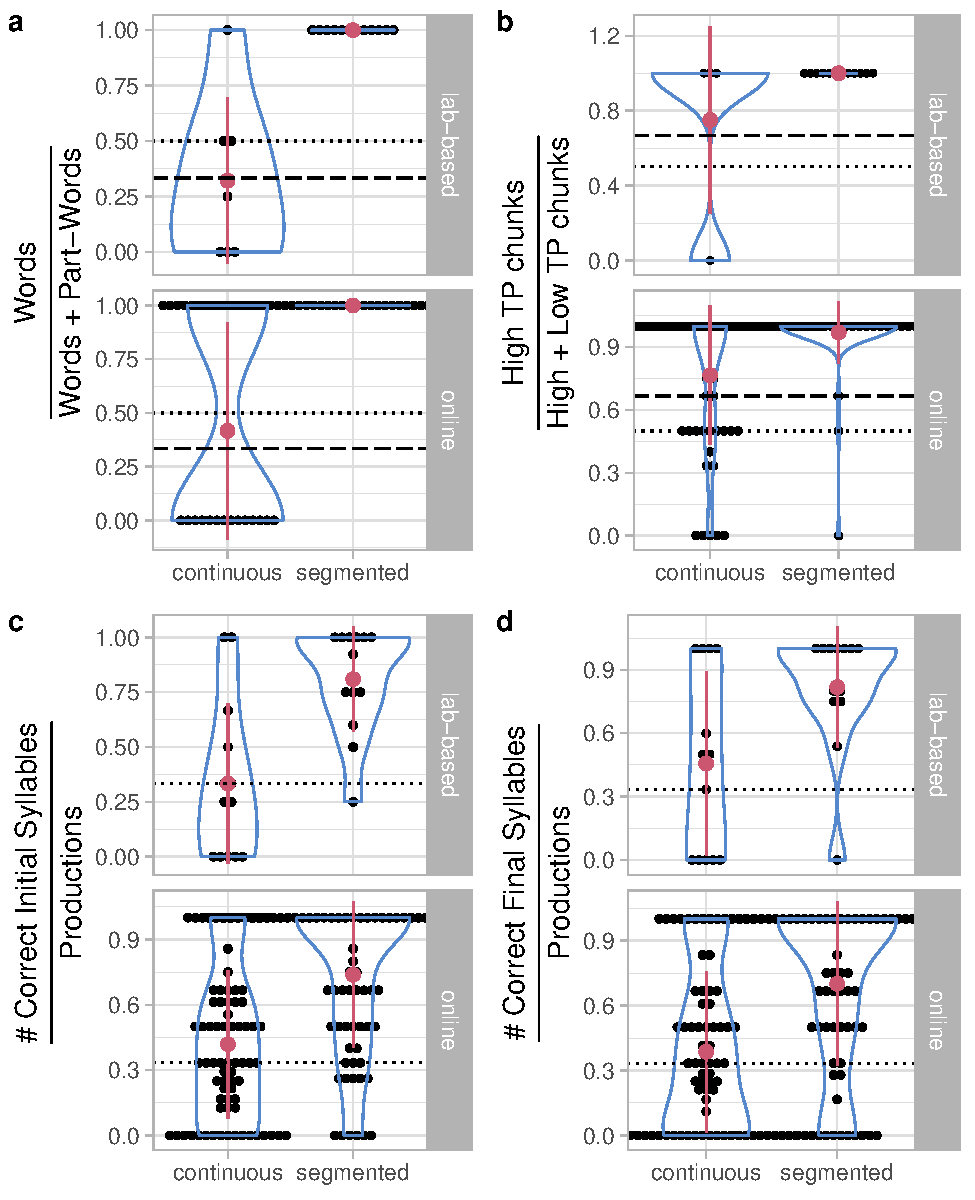
\includegraphics[width=0.8\linewidth]{segmentation_recall_combined_files/figure-latex/recall-w-pw-chunks-positions-plot-1}

}

\caption{Analyses of the participants' productions. (a) Proportion of words among words and part-words. The dotted line represents the chance level of 50\% in a two-alternative forced-choice task, while the dashed line represents the chance level of 33\% that an attested 3 syllable-chunk is a word rather than a part-word. (b) Proportion of high-TP chunks among high- and low-TP chunks. The dashed line represents the chance level of 66\% that an attested 2 syllable-chunk is a high-TP rather than a low-TP chunk. (c) proportion of productions with correct initial syllables and (d) with correct final syllables. The dotted line represents the chance level of 33\%.}\label{fig:recall-w-pw-chunks-positions-plot}
\end{figure}

\clearpage

\section{Discussion}\label{discussion}

Taken together, Experiments 1 and 2 suggest that associative learning and (declarative) memory might fulfill different computational functions. In Experiment 1, participants tracked statistical dependencies predominantly when they were embedded in a continuous speech stream, but not across pre-segmented chunk sequences. These results are consistent with Shukla et al's \citep{Shukla2007} finding that associative learning predominantly occurs within major prosodic groups, and, within these groups, predominantly at the edges of those groups; we show that, with shorter and better separated groups, associative learning can be abolished altogether. In line with results from conditioning experiments \citep{Alberts1984, Garcia1974, Gubernick1984, Martin1979}, associative learning can thus be enhanced or suppressed depending on the learning situation. The enhanced associative learning in continuous sequences 
is consistent with the view that associative learning is important for predictive processing  \citep{Turk-Browne2010, Sherman2020}, given that prediction is arguably more useful in lengthy chunks. It is also consistent with the view that associative learning may be less important for memorizing utterances, especially given that, due to its prosodic organization, speech tends to be pre-segmented into smaller groups such as those used by Shukla et al \citep{Shukla2007} or in Experiment 1 \citep{Cutler1997, Shattuck-Hufnagel1996, Brentari2011, Endress-cross-seg, Fenlon2008, Pilon1981, Christophe2001}.

Experiment 2 showed that, even when participants successfully track associative information, they remember familiarization items only when familiarized with a pre-segmented sequence; in contrast, when familiarized with a continuous sequence, their productions started with random syllables rather than actual word onsets. Given that the memory representations of linguistic items are based on their initial and final syllables \citep{Endress-Phantoms-Vision, Fischer-Baum2011}, this result thus suggests that associative learning did not lead to the creation of declarative memory representations

The combined results of Experiments 1 and 2 echo dissociations between associative learning and declarative memory. Such dissociations have long been documented behaviorally \citep{Graf1984}, developmentally \citep{Finn2016} and neuropsychologically \citep{Knowlton1996a, Rungratsameetaweemana2019, Poldrack2001, Squire1992}, to the extent that statistical predictions can \emph{impair} declarative memory encoding in healthy adults \citep{Sherman2020}. The standard conclusion is that the (cortical) declarative memory system might be independent of a (neostriatal) system for associative learning \citep{Knowlton1996a, Poldrack2001, Squire1992}. In line with earlier proposals \citep{Turk-Browne2010, Sherman2020}, we thus suggest that the computational function of associative learning might be distinct from that of (declarative) memory encoding, and that associative learning might be more important for predictive processing. The relative salience of these mechanisms might depend on how adaptive they are for the learning problem at hand.

These results also have implications for the more specific problem of word segmentation. If learners cannot use associative learning to encode word candidates in (declarative) memory, they need to use other cues. Possible cues include using known words as delimiters for other words \citep{Bortfeld2005, Brent2001, Mersad2012}, attentional allocation to beginnings and ends of utterances \citep{Monaghan2010, Seidl2008, Shukla2007}, legal sound sequences \citep{McQueen1998, Salverda2007} and universal aspects of prosody \citep{Brentari2011, Christophe2001, Endress-cross-seg, Fenlon2008, Johnson2009, Pilon1981}. Such cues might plausible support declarative memories of words because they (but not transition-based associative information) are consistent with how linguistic sequences are encoded in declarative long-term memory, where linguistic sequences are encoded with reference to their first and their last element \citep{Endress-Phantoms-Vision, Fischer-Baum2011}. 

Taken together, associative learning and declarative memory might thus have separable functions, the former for predictive processing and the latter for remembering objects and episodes.

\clearpage

\section{Methods summary}

Unless otherwise stated, stimuli were synthesized using mbrola \citep{mbrola} and the \emph{us3} (American English male) voice. Lab-based experiments were run using Psyscope X (\url{http://psy.ck.sissa.it}) in a quiet room. Online experiments were run on \url{https://testable.org}.

\subsection{Participants}\label{participants}

In Experiment 1, 30, 30 and 31 participants were retained for analysis for the pre-segmented condition, the continuous condition and its replication. In Experiment 2, 26 participants were retained for the lab-based version, and 157 for the online version. Participants reported to be native speakers of English.

\subsection{Experiment 1}

Participants were instructed to listen to a monologue in ``Martian'', and to remember the Martian words. Following this, they listened to a sequence of tri-syllabic words (Language 1: \emph{w3:legu:}, \emph{w3:levOI}, \emph{w3:lenA:}, \emph{faIzO:gu:}, \emph{faIzO:vOI}, \emph{faIzO:nA:}, \emph{rVb\{gu:}, \emph{rVb\{vOI}, \emph{rVb\{nA:}; Language 2: \emph{w3:legu:}, \emph{faIlegu:}, \emph{rVlegu:}, \emph{w3:zO:vOI}, \emph{faIzO:vOI}, \emph{rVzO:vOI}, \emph{w3:b\{nA:}, \emph{faIb\{nA:}, \emph{rVb\{nA:}). In Language 1 and 2, both TPs and the chunk frequency favored \emph{AB+C} and \emph{A+BC} patterns, respectively (TPs of 1.0 vs.~1/3; see main text). Segments lasted 60 ms and had an \(F_0\) of 120 Hz. Sequences (45 repetitions/word) were either continuous or had 540 ms silences between words. Sequences were then played thrice (total familiarization: 7 min 17s (continuous); 18 min 14 s (pre-segmented)).

Following this familiarization, participants listened to pairs of items and had to choose the more ``Martian'' one. One item comprised the \emph{first two} syllables of a word, one the \emph{last two} syllables. The three items of each kind were combined into 9 test pairs. The test pairs were presented twice.

\subsection{Experiment 2}

Participants were instructed to listen to a monologue in ``Martian'', and to remember the Martian words. The languages were those from \citet{Saffran-Science} Experiment 2 (Language 1: \emph{pAbiku}, \emph{tibudO}, \emph{dArOpi}, \emph{gOLAtu}; Language 2: \emph{bikuti}, \emph{pigOLA}, \emph{tudArO}, \emph{budOpA}). Segments lasted 108 ms at an \(F_0\) of 120 Hz. The words were combined into 20 sequences (45 repetitions/word) with different random orders, either continuously or with 222 ms silences between words. Sequences were played twice (total familiarization: 3 min 53 (continuous) and 5 min 13 (pre-segmented)). Online participants watched a nebula during familiarization.

Following the familiarization and a 30 s filled retention interval, participants completed the recall test. Lab-based participants had 45 s to repeat back the words they remembered; their vocalizations were recorded for offline analysis. Online participants had 60 s to type their answer into a comment field. Finally, participants completed a recognition test during which we pitted words against part-words.

\subsection{Analysis of productions}\label{analysis-of-productions}

The responses were transformed using a set of substitutions rules to allow for misperceptions (e.g., confusion between /b/ and /p/) or orthographic variability (e.g., \emph{ea} and \emph{ee} both reflect the sound /i/). Finally, we selected the best matches to the familiarization stimuli (see SI \ref{app:recall_analysis_steps}).

\clearpage

\bibliography{/Users/endress/ansgar.bib,/Users/endress/ansgar.own.bib}

\clearpage


\myappendix

\appsectionFirst{Methods}\label{app:methods}

\subsection{Recognition experiment}\label{recognition-experiment-london}

\subsubsection{Participants}\label{participants-1}

\begin{table}[hbp]

\caption{\label{tab:stats-london-demographics-print}Demographics of the final sample for Experiment 1.}
\centering
\begin{tabular}[t]{lrrrrl}
\toprule
Familiarization Condition & $N$ & Females & Males & Age (\M) & Age (range)\\
\midrule
Pre-segmented & 30 & 18 & 12 & 26.3 & 18-43\\
Continuous (1) & 32 & 26 & 6 & 20.1 & 18-44\\
Continuous (2) & 30 & 20 & 10 & 23.2 & 18-36\\
\bottomrule
\end{tabular}
\end{table}

Participants were recruited from the City, University London participant pool and received course credit or monetary compensation for their time. We targeted 30 participants per experiment (15 per language). The final demographic information is given in Table \ref{tab:stats-london-demographics-print}. An additional six participants took part in the experiment but were not retained for analysis because they had taken part in a prior version of this experiment (\(N = 4\)), were much older than the rest of our sample (\(N = 2\)), or used their phone during the experiment or were visibly inattentive (\(N = 2\)). Participants reported to be native speakers of English.

\subsubsection{Design}

Participants were familiarized with a sequence of tri-syllabic words. In Language 1, both the TPs and the chunk frequency was higher in the bigram formed by the first two syllables than in the bigram formed by the last two syllables; as a result, an associative learner should split a triplet like \emph{ABC} into an initial \emph{AB} chunk followed by a singleton \emph{C} syllable (hereafter \emph{AB+C} pattern). In Language 2, both the TPs and the chunk frequency favored an \emph{A+BC} pattern. The basic structure of the words is shown in Table \ref{tab:stats-london-print-language-structure}.

\begin{table}[hbp]

\caption{\label{tab:stats-london-print-language-structure}Design of Experiment 1. (Left) Language structure. (Middle) Structure of test items. Correct items for Language 1 are foils for Language 2 and vice versa. (Right) Actual items in SAMPA format; dashes indicate syllable boundaries.}
\centering
\begin{tabular}[t]{llllll}
\toprule
\multicolumn{2}{c}{Word structure for} & \multicolumn{2}{c}{Test item structure for} & \multicolumn{2}{c}{Actual words for} \\
Language 1 & Language 2 & Language 1 & Language 2 & Language 1 & Language 2\\
\midrule
ABC & ABC & AB & BC & w3:-le-gu: & w3:-le-gu:\\
ABD & FBC & FG & GD & w3:-le-vOI & faI-le-gu:\\
ABE & HBC & HJ & JE & w3:-le-nA: & rV-le-gu:\\
FGC & AGD &  &  & faI-zO:-gu: & w3:-zO:-vOI\\
FGD & FGD &  &  & faI-zO:-vOI & faI-zO:-vOI\\
\addlinespace
FGE & HGD &  &  & faI-zO:-nA: & rV-zO:-vOI\\
HJC & AJE &  &  & rV-b\{-gu: & w3:-b\{-nA:\\
HJD & FJE &  &  & rV-b\{-vOI & faI-b\{-nA:\\
HJE & HJE &  &  & rV-b\{-nA: & rV-b\{-nA:\\
\bottomrule
\end{tabular}
\end{table}

As result, in Language 1, the first bigram has a (forward and backward) TP of 1.0, while the second bigram has a (forward and backward) TP of .33. In contrast, in Language 2, the first bigram has a forward TP of .33, while the second bigram has a forward TP of 1.0. Likewise, the initial bigrams were three times as frequent as the final ones for Language 1, while the opposite holds for Language 2.

We asked whether participants would extract initial bigrams or final bigrams. The test items are given in Table \ref{tab:stats-london-print-language-structure}.

\subsubsection{Stimuli}\label{stimuli}

Stimuli were synthesized using the \emph{us3} (American English male) voice from mbrola \citep{mbrola}. (We also used the \emph{en1} (British English male) voice; however, as discussed below, this voice turned out to be of relatively low quality and introduced confounds in the data.)

Segments had a constant duration of 60 ms (syllable duration 120 ms) with a constant \(F_0\) of 120 Hz. These values were chosen to match recordings of natural speech that were intended to be used in investigations of prosodic cues to word segmentation.

For continuous streams, a single file with 45 repetitions of each word was synthesized for each language (2 min 26 s duration). It was faded in and out for 5 s using sox (\url{http://sox.sourceforge.net/}) and then compressed to an mp3 file using ffmpeg (\url{https://ffmpeg.org/}). The stream was then presented 3 times to a participant (total familiarization duration 7 min 17 s). The random order of the words was different for every participant.

For segmented streams, words were individually synthesized using mbrola. We then used a custom-made Perl script to randomize the words for each participant and concatenate them into a familiarization file using sox. The order of words was then randomized for each participant and concatenated into a single aiff file using sox. The silence among words was 540 ms (1.5 word durations). The total stream duration was 6 min 12s. The stream was then presented 3 times to a participant (total familiarization: 18 min 14 s).

\subsubsection{Apparatus}\label{apparatus}

The experiment was run using Psyscope X (\url{http://psy.ck.sissa.it}). Stimuli were presented over headphones in a quiet room. Responses were collected from pre-marked keys on the keyboard.

\subsubsection{Procedure}\label{procedure}

Participants were informed that they would listen to a monologue by a talkative Martian, and instructed to try to remember the Martian words. Following this, they listened to three repetitions of the familiarization stream described above, for a total familiarization duration of 7 min 17 s (continuous stream) or 18 min 14 s (segmented stream).

Following this familiarization, participants were presented with pairs of items with an inter-stimulus interval of 500 ms, and had to choose which items was more like what they heard during familiarization. One item comprised the first two syllables of a word, and was a correct choice for Language 1. The other items comprised the last two syllables of a word, and was a correct choice for Language 2. There were three items of each kind. They were combined into 9 test pairs. The test pairs were presented twice, with different item orders, for a total of 18 test trials.

\subsection{Recall experiment}\label{recall-experiment}

\subsubsection{Materials}\label{materials}

We re-synthesized the languages used in \citet{Saffran-Science} Experiment 2. The four words in each language are given in Table \ref{tab:recall-languages}. Stimuli were synthesized using the us3 (male American English) voice of the mbrola synthesizer \citep{mbrola}, at a constant \(F_0\) of 120 Hz and at a rate of 216 ms per syllable (108 ms per phoneme).

\begin{table}[hbp]

\caption{\label{tab:recall-print-languages}\label{tab:recall-languages}Languages used Experiment 2. The words are the same as in \cite{Saffran-Science} Experiment 2.}
\centering
\begin{tabular}[t]{ll}
\toprule
L1 & L2\\
\midrule
pabiku & bikuti\\
tibudo & pigola\\
daropi & tudaro\\
golatu & budopa\\
\bottomrule
\end{tabular}
\end{table}

During familiarization, words were presented 45 times each. We generated random concatenations of 45 repetitions of the 4 words, with the constraint that words could not occur in immediate repetition. Each randomization was then (i) synthesized into a continuous speech stream using mbrola and then converted to mp3 using ffmpeg (\url{https://ffmpeg.org/}) (ii) used to concatenate words that had been synthesized in isolation, separated by silences of 222 ms into a segmented speech stream, which was then converted to mp3. Streams were faded in and out for 5 s using sox (\url{http://sox.sourceforge.net/}). For continuous streams, this yielded a stream duration of 1 min 57 s; for segmented streams, the duration was 2 min 37.

We created 20 versions of each stream with different random orders of words.

\clearpage

\subsubsection{Procedure}\label{procedure-1}

\paragraph{Familiarization}\label{familiarization}

Participants were informed that they would be listening to an unknown language and that they should try to learn the words from that language. Following, the familiarization stream was presented twice, leading to a total familiarization duration of 3 min 53 for the continuous streams and 5 min 13 for the segmented streams. They could proceed to the next presentation of the stream by pressing a button.

For the online experiments, participants watched a video with no clear objects during the familiarization (panning of the Carina nebula, obtained from \url{https://esahubble.org/videos/heic0707g/}). The video was combined with the speech stream using the muxmovie utility.

Following the familiarization, there was a 30 s retention interval. In both the lab-based and the online experiments, participants were instructed to count backwards from 99 in time with a metronome beat at 3s / beat. Performance was not monitored.

\paragraph{Recall test}\label{recall-test}

Following the retention interval, participants completed the recall test. During the lab-based experiments, participants had 45 s to repeat back the words they remembered; their vocalizations were recorded using ffmpeg and saved in mp3 format. During the web-based experiments, participants had 60 s to type their answer into a comment field, during which they viewed a progress bar.

\paragraph{Recognition test}\label{recognition-test}

Following the recall test, participant completed a recognition test during which we pitted words against part-words. The (correct) test words for Language 1 (and part-words for Language 2) were /pAbiku/ and /tibudO/; the (correct) test words for Language 2 (and part-words for Language 1) were /tudArO/ and /pigOlA/. These items were combined into 4 test pairs.

\appsection{Analysis}\label{app:analysis}

\subsection{Recognition tests}\label{recognition-tests}

Accuracy was averaged for each participant, and the scores were tested against the chance level of 50\% using Wilcoxon tests. Performance differences across the languages (Language 1 vs.~2) and, when applicable, familiarization conditions (pre-segmented vs.~continuous) were assessed using a generalized linear mixed model for the trial-by-trial data with the fixed factors language and, where applicable, familiarization condition, as well as random slopes for participants, correct items and foils. Following \citep{Baayen2008}, random factors were removed from the model when they did not contribute to the model likelihood.

We use likelihood ratios to provide evidence for the null hypothesis that performance did not differ from the chance level of 50\%. Following \citep{Glover2004}, we fit the participant averages to (i) a linear model comprising only an intercept and (ii) the null model fixing the intercept to the appropriate baseline level, and evaluated the likelihood of these models after correcting for the difference in the number of parameters using the Bayesian Information Criterion.

\subsection{Recall test}\label{app:recall_analysis}

\subsubsection{Analysis procedure}\label{app:recall_analysis_steps}

Participants in Experiment 2 had to recall what they remembered from the familiarization streams. Lab-based participants were recorded and their productions were transcribed by two independent observers. Disagreements were resolved by discussion. Online participants typed their responses directly into a comment box. We then applied a number of substitution rules to allow for misperceptions (e.g., a confusion between /p/ and /b/) and orthographic variability (e.g., \emph{tea} and \emph{tee} are both pronounced as /ti/). The complete list of substitution rules is shown in Table \ref{tab:recall-print-substitution-rules}.

Each recall response was analyzed in five steps. First, we applied pre-segmentation substitution rules to make the transcriptions more consistent (see Table \ref{tab:recall-print-substitution-rules}, ``before segmentation''). For example, \emph{ea} (presumably as in \emph{tea}) was replaced with \emph{i}. These substitutions were not considered when calculating the derivation length (see below).

Second, responses were segmented into their underlying units. If the response did not contain any commata (,) or semicolons (;), any spaces in the response were used to delineate units. If a response contained a semicolon or comma, these were used to delineate units. For each of the resulting units, we verified if they contained additional spaces. If they did, these spaces were removed if further segmenting the units based on the spaces resulted in one or more single-syllable units (operationalized as a string with a single vowel); otherwise, the units were further sub-divided based on the spaces. The rationale for this algorithm is that responses such as \emph{bee coo tee,two da ra,bout too pa} were likely to reflect the words \emph{bikuti}, \emph{tudaro} and \emph{budopa}.

Third, we removed geminate consonants and applied another set of substitution rules to take into account possible misperceptions (see Table \ref{tab:recall-print-substitution-rules}). For example, we treated the voiced and unvoiced variety of stop consonants as interchangeable. Specifically, for each ``\emph{surface}'' form produced by the participants, we generated candidate ``\emph{underlying}'' forms by recursively applying all substitutions rules and keeping track of the number of substitution rules that were applied to derive an underlying form from a surface form. For each unique candidate underlying form, we kept the shortest derivation.

Fourth, for each candidate underlying form, we identified the longest matching string in the familiarization stream. The algorithm first verified if a form was contained in a speech stream starting with an \emph{A}, \emph{B} or \emph{C} syllable; if the underlying form contained unattested syllable, one syllable change was allowed with respect to the speech streams. If no matches were found, two sub-strings were created by clipping the first or the last syllable from the underlying form, and the search was repeated recursively for each of these sub strings until a match was found. We then selected the longest match for all sub strings.

Fifth, for each surface form, we selected the underlying form among the candidate underlying forms using three criteria:

\begin{enumerate}
\def\labelenumi{\arabic{enumi}.}
\tightlist
\item
The winning underlying form had had the maximal \emph{number of attested syllables} among candidate underlying forms;
\item
The winning underlying form had the \emph{maximal length} among candidate underlying forms;
\item
The winning underlying form had the \emph{shortest derivation} among candidate underlying forms.
\end{enumerate}

The criteria were applied in this order.

\paragraph{Substitution rules compensating for potential misperceptions}\label{substitution-rules-compensating-for-potential-misperceptions}

All substitution rules are listed in Table \ref{tab:recall-print-substitution-rules}. We now motivate the substitution rules compensating for potential misperceptions:

\begin{itemize}
\tightlist
\item
  /O/ might be perceived as /A/
\item
Voiced and unvoiced consonants can be confused; that is /g/ can be confused with /k/, /d/ with /t/ and /b/ and /p/.
\item
  /b/ might be perceived as /v/.
\end{itemize}

In some cases, these rules result in multiple possible matches. For example, the transcription \emph{rapidala} might correspond to /rOpidAlA/ or /rOpidOlA/.

In such cases, we apply the following criteria (in the following order) to decide which match to choose.

\begin{enumerate}
\def\labelenumi{\arabic{enumi}.}
\tightlist
\item
Choose the option leading to more or longer chunks that are attested in the speech stream.
\item
If multiple options lead to chunks of equal length, choose the option requiring fewer changes with respect to the original transcription.
\end{enumerate}

\begin{table}

\caption{\label{tab:recall-print-substitution-rules}Substitution rules applied to the participants vocalizations before and after the input was segmented into chunks. The patterns are given as Perl regular expressions. Substitutions prior to segmentation were not counted when calculating the derivation length.}
\centering
\begin{tabular}[t]{llll}
\toprule
\multicolumn{2}{c}{Before segmentation} & \multicolumn{2}{c}{After segmentation} \\
\cmidrule(l{3pt}r{3pt}){1-2} \cmidrule(l{3pt}r{3pt}){3-4}
Pattern & Replacement & Pattern & Replacement\\
\midrule
\textbackslash{}.\{3,\} &  & u & o\\
- &  & v & b\\
2 & tu & p & b\\
two & tu & b & p\\
([aeou])ck & \textbackslash{}1k & t & d\\
\addlinespace
ar([,\textbackslash{}s+]) & a\textbackslash{}1 & d & t\\
ar\$ & a & k & g\\
tyu & tu & g & k\\
ph & f & a & o\\
th & t &  & \\
\addlinespace
qu & k &  & \\
ea & i &  & \\
ou & u &  & \\
aw & a &  & \\
ai & a &  & \\
\addlinespace
ie & i &  & \\
ee & i &  & \\
oo & u &  & \\
e & i &  & \\
c & k &  & \\
\addlinespace
w & v &  & \\
y & i &  & \\
h &  &  & \\
\bottomrule
\end{tabular}
\end{table}

\subsubsection{Measures of interest}\label{measures-of-interest}

We computed various properties for each underlying form, given the ``target'' language the participant had been exposed to. All measures provided in the raw data are described in Table \ref{tab:recall-print-used-column-attributes}.

\begin{table}[!h]

\caption{\label{tab:recall-print-used-column-attributes}Analyses performed for the vocalizations}
\centering
\resizebox{\linewidth}{!}{
\begin{tabular}[t]{l>{\raggedright\arraybackslash}p{30em}}
\toprule
Column name in data file & Meaning\\
\midrule
n.items & Number of recalled items\\
n.syll & Mean number of syllables of the recalled items\\
n.words & Number of recalled words\\
p.words & Proportion (among recalled items) of words\\
n.words.or.multiple & Number of recalled words or concatenation of words\\
\addlinespace
p.words.or.multiple & Proportion (among recalled items) of words or concatenation of words\\
n.part.words & Number of recalled part-words\\
p.part.words & Proportion (among recalled items) of part-words\\
n.part.words.or.multiple & Number of recalled part-words or concatenation of part-words\\
p.part.words.or.multiple & Proportion (among recalled items) of part-words or concatenation of part-words\\
\addlinespace
p.words.part.words & Proportion of words among (recalled) words and part-words. This is used for comparison to the recognition test.\\
p.words.part.words.or.multiple & Proportion of words among (recalled) words and part-words or concatenation thereof. This is used for comparison to the recognition test.\\
n.high.tp.chunk & Number of high TP chunks. High TP chunks are defined as two-syllabic chunk from a word\\
p.high.tp.chunk & Proprtion (among recalled items) of high TP chunks. High TP chunks are defined as two-syllabic chunk from a word\\
n.low.tp.chunk & Number of low TP chunks. Low TP chunks are defined as two-syllabic word transitions\\
\addlinespace
p.low.tp.chunk & Proportion (among recalled items) of low TP chunks. Low TP chunks are defined as two-syllabic word transitions\\
p.high.tp.chunk.low.tp.chunk & Proportion of high-TP chunks among high and low-TP chunks. High TP Chunks are defined as two-syllabic chunks from words; low TP chunks are two-syllabic word transitions\\
average\_fw\_tp & Average (across recalled items) of average forward TPs among transitions in a given item.\\
average\_fw\_tp\_d\_actual\_expected & Average (across recalled items) of the difference between the average ACTUAL forward TPs among transitions in a given item and the EXPECTED forward TP in that item, based on the items first element. See calculate.expected.tps.for.chunks for the calculations\\
average\_bw\_tp & Average (across recalled items) of average backward TPs among transitions in a given item.\\
\addlinespace
p.correct.initial.syll & Proportion (among recalled items) that have a correct initial syllable.\\
p.correct.final.syll & Proportion (among recalled items) that have a correct final syllable.\\
p.correct.initial.or.final.syll & Proportion (among recalled items) that have a correct initial or final syllable.\\
\bottomrule
\end{tabular}}
\end{table}


\paragraph{Measures}\label{measures}

For each underlying form, we calculate:

\begin{enumerate}
\def\labelenumi{\arabic{enumi}.}
\tightlist
\item
  the number of syllables;
\item
  whether it was a word from the target language;
\item
  whether it was a concatenation of words from the target language;
\item
whether it was a single word or a concatenation of words from the target language (i.e., the disjunction of (2) and (3));
\item
  whether it was a part-words from the target language,
\item
whether it was a \emph{complete} concatenation of part-words from the target language (i.e., the number of syllables of the item had to be a multiple of three, without any unattested syllables);
\item
whether it was a single part-word or a concatenation of part-words from the target language;
\item
whether it was high-TP chunk (i.e., a word with the first or the last syllable missing, after removing any leading or trailing unattested syllables);
\item
  whether it was a low-TP chunk (i.e., a chunk of the form \(C_iA_j\), after removing lead or trailing unattested syllables;
\item
  whether it had a ``correct'' initial syllable
\item
  whether it had a ``correct'' final syllable;
\item
whether it is part of the speech stream (i.e., the disjunction of being an attested syllable, being a word or a concatenation thereof, being a part-word or a concatenation thereof, being a high-TP chunk or a low-TP chunk);
\item
  the average forward TP of the transitions in the form;
\item
the \emph{expected} forward TP of the form if form is attested in the speech stream (see below for the calculation);
\item
  the average backward TP of the transitions in the form.
\end{enumerate}

\paragraph{Expected TPs}\label{expected-tps}

For items that are \emph{correctly} reproduced from the speech stream, the expected TPs depend on the starting position. For example, the expected TPs for items of at least 2 syllables starting on an initial syllable are (1, 1, 1/3, 1, 1, 1/3, 1, 1, 1/3, \ldots{}); if the item starts on a word-medial syllable, these TPs are (1, 1/3, 1, 1, 1/3, 1, 1, 1/3, 1, \ldots{}).

In contrast, the expected TPs for a random concatenation of syllables are the TPs in a random bigram. For an \emph{A} or a \emph{B} syllable, the random TP is 1 \(\times\) 1 / 12, as there is only 1 (out of 12) non-zero TP continuations. For a C syllable, the random TP is 3 \(\times\) 1/3 / 12, as there are 3 possible concatenations. On average, the random TP is thus \((1/12 + 1/12 + 1/12)/ 3 = 1/12 \approx .083\).

\paragraph{Exclusion of responses and participants}\label{exclusion-of-responses-and-participants}

There was a considerable number of recall responses containing unattested syllables. The complete list of unattested items is in \texttt{segmentation\_recall\_unattested.xlsx} in the supplementary data. Unattested items are items that are not words, part-words (or concatenations thereof), high- or low-TP chunks, or a single syllable. However, it is unclear if these unattested syllables reflect misperceptions not caught by our substitution rules, typos, memory failures or creative responses. This makes it difficult to analyze these responses. For example, the TPs from and to an unattested syllable are zero. However, if the unattested syllable reflects a misperception or a typo, the true TP would be positive, and our estimates would underestimate the participant's statistical learning ability.

Here, we decided to include items with unattested syllables to avoid excluding an excessive number of participants. However, the results after removing such items are essentially identical, with the exception of the TPs in the participants' responses. Given that TPs to and from unattested syllables are zero by definition, TPs after removal of responses containing unattested syllables are much higher.

We also decided to remove single syllable responses, as it is not clear if participants volunteered such responses because they thought that individual syllables reflected the underlying units in the speech streams or because they misunderstood what they were ask to do.

\subsubsection{Demographics}

To reduce performance differences between the pre-segmented and the continuous familiarization conditions, participants were excluded from analysis if their accuracy in the recognition test was below 50\% (\emph{N} = 19). Another 11 participants were excluded because parsing their productions took an excessive amount of computing time, though their productions did not seem to resemble the familiarization items in the first place. The final demographic information is given in Table \ref{tab:recall-final-demographics-print}.

\begin{table}

\caption{\label{tab:recall-final-demographics-print}Demographics of the final sample. The lab-based participants completed both segmentation conditions.}
\centering
\begin{tabular}[t]{llrrrrl}
\toprule
Sequence Type & Language & N & Females & Male & Age (\M) & Age (range)\\
\midrule
\addlinespace[0.3em]
\multicolumn{7}{l}{\textbf{Lab-based}}\\
\hspace{1em}continuous & both & 13 & 13 & 0 & 17.8 & 0-22\\
\hspace{1em}segmented & both & 13 & 13 & 0 & 17.8 & 0-22\\
\addlinespace[0.3em]
\multicolumn{7}{l}{\textbf{Online}}\\
\hspace{1em}continuous & L1 & 38 & 8 & 30 & 31.7 & 18-71\\
\hspace{1em}continuous & L2 & 38 & 18 & 20 & 29.7 & 19-71\\
\hspace{1em}segmented & L1 & 38 & 11 & 27 & 28.8 & 18-55\\
\hspace{1em}segmented & L2 & 38 & 4 & 34 & 29.0 & 18-62\\
\bottomrule
\end{tabular}
\end{table}

\clearpage

\appsection{Additional results}
\subsection{Experiment 1}

\begin{table}[hb]

\caption{\label{tab:stats-london-stats.us.lang.glmm.print}Performance differences across familiarization conditions in Experiment 1. The differences were assessed using a generalized linear model for the trial-by-trial data, using participants, correct items and foils as random factors. Random factors were removed from the model when they did not contribute to the model likelihood.}
\centering
\begin{tabular}[t]{lrrlrr}
\toprule
Effect & Estimate & Std. Error & CI & \T & \p\\
\midrule
\addlinespace[0.3em]
\multicolumn{6}{l}{\textbf{Pre-segmented familiarization}}\\
\hspace{1em}Language = L2 & 0.114 & 0.673 & -1.2, 1.43 & 0.170 & 0.865\\
\addlinespace[0.3em]
\multicolumn{6}{l}{\textbf{Continuous familiarization (1)}}\\
\hspace{1em}Language = L2 & -0.184 & 0.480 & -1.12, 0.757 & -0.383 & 0.702\\
\addlinespace[0.3em]
\multicolumn{6}{l}{\textbf{Continuous familiarization (2)}}\\
\hspace{1em}Language = L2 & 0.317 & 0.786 & -1.22, 1.86 & 0.403 & 0.687\\
\addlinespace[0.3em]
\multicolumn{6}{l}{\textbf{Pre-segmented vs. continuous familiarization (1)}}\\
\hspace{1em}Language = L2 & -0.019 & 0.557 & -1.11, 1.07 & -0.033 & 0.973\\
\hspace{1em}Pre-segmentation: Yes & -0.328 & 0.188 & -0.696, 0.0391 & -1.752 & 0.080\\
\addlinespace[0.3em]
\multicolumn{6}{l}{\textbf{Pre-segmented vs. continuous familiarization (2)}}\\
\hspace{1em}Language = L2 & 0.215 & 0.657 & -1.07, 1.5 & 0.327 & 0.743\\
\hspace{1em}Pre-segmentation: Yes & -0.608 & 0.244 & -1.09, -0.13 & -2.493 & 0.013\\
\bottomrule
\end{tabular}
\end{table}

\clearpage

\subsection{Experiment 2}\label{additional-results-for-the-recall-experiments}

\subsubsection{Additional tables and figures}\label{additional-tables-and-figures}

\begin{table}[hb]

\caption{\label{tab:recall-extra-results-print}Various supplementary analyses pertaining to the productions as well as test against their chances levels.}
\centering
\resizebox{\linewidth}{!}{
\begin{tabular}[t]{l>{\raggedright\arraybackslash}p{20em}>{\raggedright\arraybackslash}p{20em}>{\raggedleft\arraybackslash}p{15em}}
\toprule
 & Continuous & Segmented & \p (Continuous vs. Segmented). \\
\midrule
\addlinespace[0.3em]
\multicolumn{4}{l}{\textbf{Number of words}}\\
\hspace{1em}lab-based & \M = 0.308, \SE = 0.139, \p = 0.0719 & \M = 1.85, \SE = 0.308, \p = 0.00224 & 0.005\\
\hspace{1em}online & \M = 0.224, \SE = 0.0791, \p = 0.00482 & \M = 1.32, \SE = 0.143, \p = 7.32e-11 & < 0.001\\
\addlinespace[0.3em]
\multicolumn{4}{l}{\textbf{Proportion of words among productions}}\\
\hspace{1em}lab-based & \M = 0.308, \SE = 0.139, \p = 0.0719 & \M = 1.85, \SE = 0.308, \p = 0.00224 & 0.005\\
\hspace{1em}online & \M = 0.224, \SE = 0.0791, \p = 0.00482 & \M = 1.32, \SE = 0.143, \p = 7.32e-11 & < 0.001\\
\addlinespace[0.3em]
\multicolumn{4}{l}{\textbf{Number of part-words}}\\
\hspace{1em}lab-based & \M = 0.692, \SE = 0.273, \p = 0.031 & \M = 0, \SE = 0, \p = NaN & 0.031\\
\hspace{1em}online & \M = 0.25, \SE = 0.0657, \p = 0.000717 & \M = 0, \SE = 0, \p = NaN & < 0.001\\
\addlinespace[0.3em]
\multicolumn{4}{l}{\textbf{Proportion of part-words among productions}}\\
\hspace{1em}lab-based & \M = 0.692, \SE = 0.273, \p = 0.031 & \M = 0, \SE = 0, \p = NaN & 0.031\\
\hspace{1em}online & \M = 0.25, \SE = 0.0657, \p = 0.000717 & \M = 0, \SE = 0, \p = NaN & < 0.001\\
\addlinespace[0.3em]
\multicolumn{4}{l}{\textbf{Actual vs. expected forward TPs}}\\
\hspace{1em}lab-based & \M = -0.462, \SE = 0.07, \p = 0.000244 & \M = -0.315, \SE = 0.0803, \p = 0.00915 & 0.147\\
\hspace{1em}online & \M = -0.42, \SE = 0.0329, \p = 1.3e-12 & \M = -0.352, \SE = 0.0365, \p = 7.56e-11 & 0.120\\
\addlinespace[0.3em]
\multicolumn{4}{l}{\textbf{Number of High-TP chunks}}\\
\hspace{1em}lab-based & \M = 0.769, \SE = 0.459, \p = 0.181 & \M = 2.31, \SE = 0.361, \p = 0.00224 & 0.022\\
\hspace{1em}online & \M = 1.13, \SE = 0.13, \p = 5.35e-10 & \M = 1.62, \SE = 0.147, \p = 6.19e-12 & 0.014\\
\addlinespace[0.3em]
\multicolumn{4}{l}{\textbf{Proportion of High-TP chunks among productions}}\\
\hspace{1em}lab-based & \M = 0.104, \SE = 0.0601, \p = 0.181 & \M = 0.615, \SE = 0.0999, \p = 0.00241 & 0.003\\
\hspace{1em}online & \M = 0.279, \SE = 0.0331, \p = 1.08e-09 & \M = 0.516, \SE = 0.0435, \p = 8.27e-12 & < 0.001\\
\addlinespace[0.3em]
\multicolumn{4}{l}{\textbf{Number of Low-TP chunks}}\\
\hspace{1em}lab-based & \M = 0.0769, \SE = 0.0801, \p = > .999 & \M = 0, \SE = 0, \p = NaN & > .999\\
\hspace{1em}online & \M = 0.355, \SE = 0.0747, \p = 2.41e-05 & \M = 0.0395, \SE = 0.0226, \p = 0.149 & < 0.001\\
\addlinespace[0.3em]
\multicolumn{4}{l}{\textbf{Number of Low-TP chunks among productions}}\\
\hspace{1em}lab-based & \M = 0.011, \SE = 0.0114, \p = > .999 & \M = 0, \SE = 0, \p = NaN & > .999\\
\hspace{1em}online & \M = 0.0855, \SE = 0.0198, \p = 6.04e-05 & \M = 0.00846, \SE = 0.00523, \p = 0.181 & < 0.001\\
\bottomrule
\multicolumn{4}{l}{\textsuperscript{*} The expected TPs for items of at least 2 syllables starting on an initial syllable are 1, 1/3, 1, 1, 1/3, 1, 1, 1/3,}\\
\multicolumn{4}{l}{\textellipsis. The difference between the actual and the expected TP needs to be compared to zero, as the expected TP}\\
\multicolumn{4}{l}{differs across items.}\\
\end{tabular}}
\end{table}

\begin{figure}

{\centering 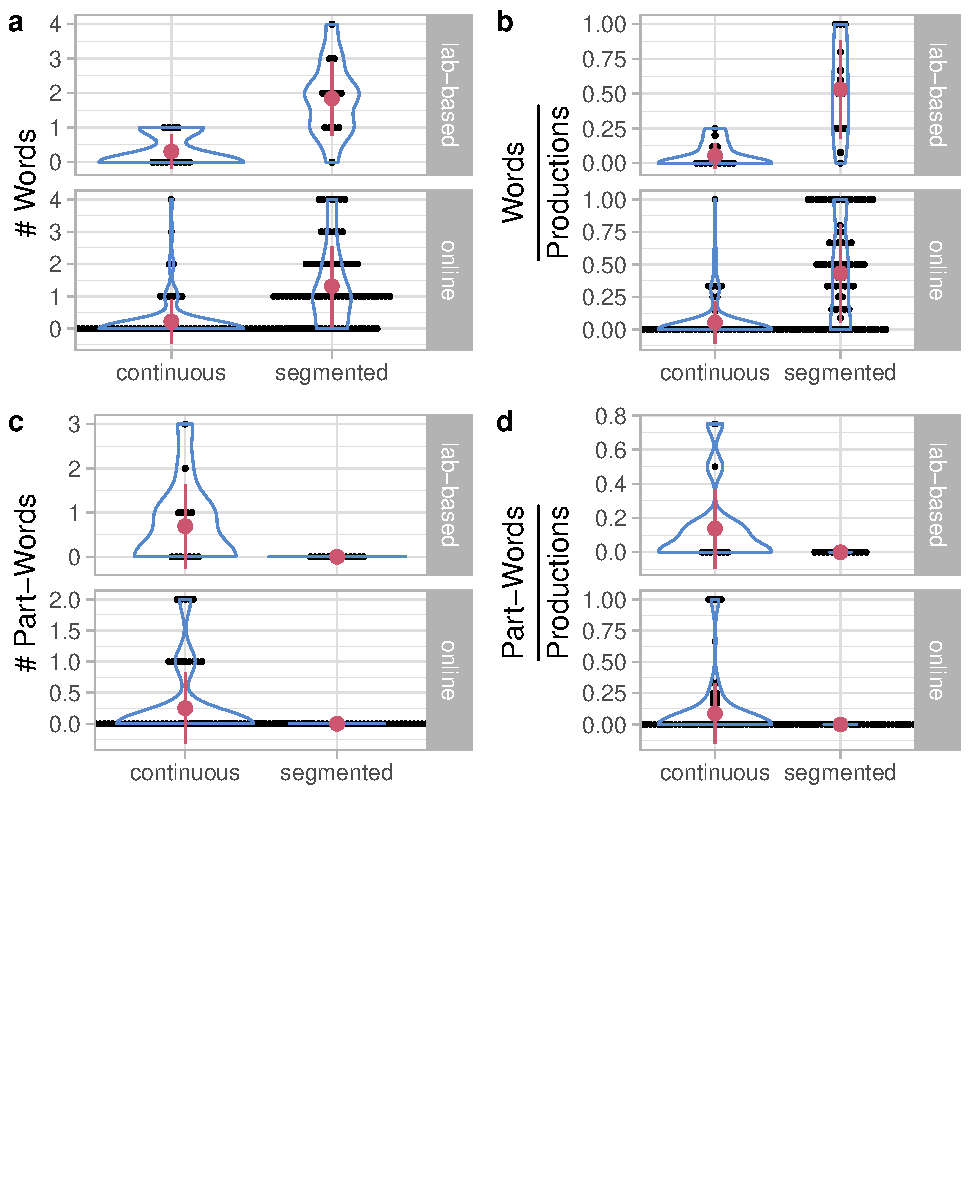
\includegraphics[width=0.8\linewidth]{segmentation_recall_combined_files/figure-latex/recall-words-part-words-raw-plot-1} 

}

\caption{Number and proportion (among vocalizations) of words and part-words.}\label{fig:recall-words-part-words-raw-plot}
\end{figure}

\begin{figure}

{\centering 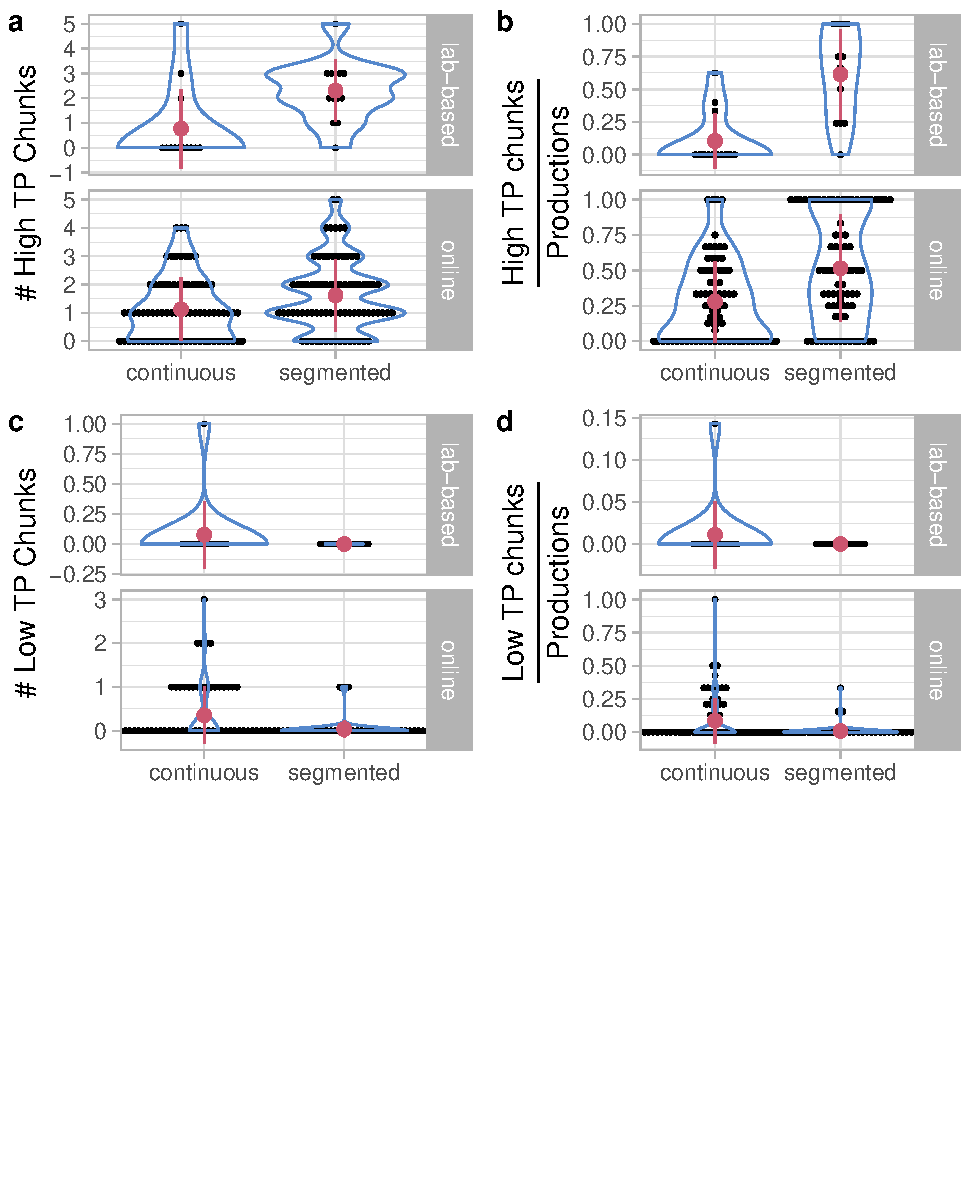
\includegraphics[width=0.8\linewidth]{segmentation_recall_combined_files/figure-latex/recall-tp-chunks-raw-plot-1} 

}

\caption{Plot of High and Low TP chunks.}\label{fig:recall-tp-chunks-raw-plot}
\end{figure}

\clearpage

\subsection{Fit of the number of participants producing words or part-words to a binomial distribution}\label{app:likelihood}

We fit the data to two models, one where the learner successfully detected word-boundaries, and one where the learner successfully track TPs but initiates productions at a random position. We then calculate the likelihood of the data given these models.

According to the first model, the probability of producing words rather then part-words is \(p^1_{\text{W}} = 1\), and the probability of using part-words is \(p^1_{\text{PW}} = 1 - p^1_{\text{W}} = 0\). According to the second model, the learner has one chance in three to initiate a production on a word-initial syllable. As a result, the probability of producing words is \(p^2_{\text{W}} = \frac{1}{3}\), and the probability of using part-words is \(p^2_{\text{PW}} = 1 - p^2_{\text{W}} = \frac{2}{3}\).

Assuming that participants produce either words or part-words, the probability of \(N_{\text{W}}\) producing words and \(N_{\text{PW}}\) producing part-words is given by a binomial distribution. We can then use Bayes' theorem to calculate the model likelihood \(P(\text{model|data}) = P(\text{data|model}) \frac{P(\text{model})}{P(\text{data})}\). If both models are equally likely a priori, the likelihood ratio of the models given the data is the likelihood ratio of the data given the models:

\begin{eqnarray*}
\Lambda_{1,2} & = & \frac{P(\text{model}_1 | \text{data})}{P(\text{model}_2 | \text{data})}
 %
 = \frac{P(\text{data} | \text{model}_1 )}{P(\text{data} | \text{model}_2)} \\
 %
 & = & \frac{\left(\begin{array}{c}
N_{\text{W}} + N_{\text{PW}}\\
N_{\text{W}}
\end{array}\right)}{\left(\begin{array}{c}
N_{\text{W}} + N_{\text{PW}}\\
N_{\text{W}}
\end{array}\right)} 
\frac{1^{N_{\text{W}}} 0^{N_{\text{PW}}}}{\frac{1}{3}^{N_{\text{W}}} \frac{2}{3}^{N_{\text{PW}}}} \\
%
& = & \left\{\begin{array}{ll}
3^{N_{\text{PW}}} & N_{\text{PW}} = 0\\
0 & N_{\text{PW}} > 0
\end{array}\right.
\end{eqnarray*}

For \(N_{\text{PW}} = 0\), the likelihood ratio in favor of the first model is \(3^{N_{\text{PW}}}\); \(N_{\text{PW}} > 0\) the likelihood ratio in favor of the second model is infinite.

\appsection{Pilot Experiment 1: Using the \emph{en1} voice}\label{app:exp_en1}

We ran an experiment identical to the pre-segmented condition of Experiment 1, except that materials were synthesized using the {\em en1} (British English male) voice. 

\subsection{Familiarization with a pre-segmented stream}\label{app:exp_en1_segm}

\begin{figure}

{\centering 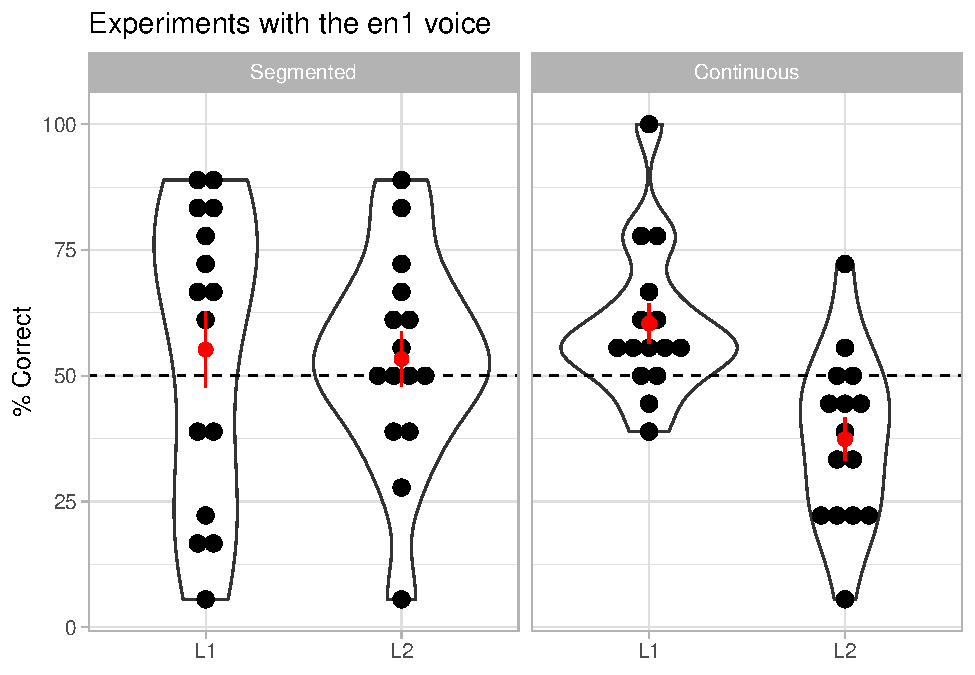
\includegraphics[width=0.8\linewidth]{segmentation_recall_combined_files/figure-latex/stats-london-stats.3x.en.segm-cont.plot-1} 

}

\caption{Results for a pre-segmented presentation of the stream (540 ms silences, left) and continuous presentation of the stream (right). Each word was repeated 45 times. The voice was {\em en1}.}\label{fig:stats-london-stats.3x.en.segm-cont.plot}
\end{figure}

\begin{table}[hpb]

\caption{\label{tab:stats-london-descriptives}Descriptives for Experiment 1 (using the {\em us3} voice) and Pilot Experiment 1 (using the {\em en1} voice).}
\centering
\begin{tabular}[t]{lrrrr}
\toprule
Condition & $N$ & \M & \SE & \p\\
\midrule
\addlinespace[0.3em]
\multicolumn{5}{l}{\textbf{us2 voice}}\\
\hspace{1em}Pre-segmented & 30 & 0.517 & 0.028 & 0.307\\
\hspace{1em}Continuous (1) & 32 & 0.585 & 0.029 & 0.018\\
\hspace{1em}Continuous (2) & 30 & 0.628 & 0.040 & 0.007\\
\addlinespace[0.3em]
\multicolumn{5}{l}{\textbf{en1 voice}}\\
\hspace{1em}Pre-segmented (en1) & 30 & 0.543 & 0.047 & 0.268\\
\hspace{1em}Continuous (en1) & 30 & 0.489 & 0.036 & 0.739\\
\bottomrule
\end{tabular}
\end{table}

As shown in Figure \ref{fig:stats-london-stats.3x.en.segm-cont.plot}, when the speech stream was pre-segmented, the average performance did not differ significantly from the chance level of 50\%, (\M~= 54.26, \SD~= 25.09), \D~= 0.17, \CI~= 44.89, 63.63, ns, . Likelihood ratio analysis favored the null hypothesis by a factor of 3.555 after correction with the Bayesian Information Criterion. Further, as shown in Table \ref{tab:stats.en.lang.glmm}, performance did not depend on the language condition.

\subsection{Familiarization with a continuous stream}\label{app:exp_en1_cont}

As shown in Figure \ref{fig:stats-london-stats.3x.en.segm-cont.plot}, when the speech stream was continuous, the average performance did not differ significantly from the chance level of 50\%, (\M~= 48.89, \SD~= 19.65), \T(29) = -0.31, \p~= 0.759, \D~= 0.057, \CI~= 41.55, 56.23, ns, \(V\) = 166, \(p\) = 0.818. Likelihood analyses revealed that the null hypothesis was 5.221 than the alternative hypothesis after a correction with the Bayesian Information Criterion. However, as shown in Table \ref{tab:stats.en.lang.glmm}, performance was much better for Language 1 than for Language 2, presumably due to some click-like sounds the synthesizer produced for some stops and fricatives (notably /f/ and /g/). These sound likely affected grouping, and prevented participants from using statistical learning.

\begin{table}

\caption{\label{tab:stats-london-stats.en.lang.glmm.print}\label{tab:stats.en.lang.glmm}Performance differences across language conditions in Pilot Experiment 1. The differences were assessed using a generalized linear model for the trial-by-trial data, using participants, correct items and foils as random factors. Random factors were removed from the model when they did not contribute to the model likelihood}
\centering
\begin{tabular}[t]{lrrlrr}
\toprule
Effect & Estimate & Std. Error & CI & \T & \p\\
\midrule
\addlinespace[0.3em]
\multicolumn{6}{l}{\textbf{Pre-segmented}}\\
\hspace{1em}Language = L2 & -0.097 & 0.441 & -0.96, 0.767 & -0.22 & 0.826\\
\addlinespace[0.3em]
\multicolumn{6}{l}{\textbf{Continuous}}\\
\hspace{1em}Language = L2 & -1.024 & 0.410 & -1.83, -0.22 & -2.50 & 0.013\\
\bottomrule
\end{tabular}
\end{table}


\appsection{Pilot Experiment 2: Testing the use of chunk frequency}\label{app:pilot_bcn}

In Pilot Experiment 2, we asked if participants could break up tri-syllabic items by using the chunk frequency of sub-chunks. The artificial languages were designed such that, in a trisyllabic item such as \emph{ABC}, chunk frequency (and backwards TPs) favor in the initial \emph{AB} chunk for half of the participants, and the final \emph{BC} chunk for the other participants.

Across participants, we also varied the exposure to the languages, with 3, 15 or 30 repetitions per word, respectively.

\subsection{Methods}

\subsubsection{Participants}

\begin{table}[hpb]

\caption{\label{tab:bcn-demographics}Demographics of Pilot Experiment 2.}
\centering
\begin{tabular}[t]{rrrl}
\toprule
\# Repetitions/word & $N$ & Age (\M) & Age (Range)\\
\midrule
3 & 37 & 21.1 & 18-35\\
15 & 41 & 21.0 & 18-27\\
30 & 40 & 20.8 & 18-26\\
\bottomrule
\end{tabular}
\end{table}

Demographic information of Pilot Experiment 2 is given in Table \ref{tab:bcn-demographics}. Participants were native speakers of Spanish and Catalan and were recruited from the Universitat Pompeu Fabra community.

\subsubsection{Stimuli}

Stimuli transcriptions are given in Table \ref{tab:bcn-print-language-structure}. They were synthesized using the \emph{es2} (Spanish male) voice of the mbrola \citep{mbrola} speech synthesized, using a segment duration of 225 ms and an fundamental frequency of 120 Hz.

\subsubsection{Apparatus}

Participants were test individually in a quiet room. Stimuli were presented over headphones. Responses were collected from pre-marked keys on the keyboard. The experiment with 3 repetitions per word (see below) were run using PsyScope X; the other experiments were run using Experyment (\url{https://www.expyriment.org/}).

\subsubsection{Familiarization}

The design of Pilot Experiment 2 is shown in Table \ref{tab:bcn-print-language-structure}. The languages comprise trisyllabic items. All forward TPs were 0.5. However, in Language 1 the chunk composed of the first two syllables (e.g., \emph{AB} in \emph{ABC}) were twice as frequent as the chunk composed of the last two syllables (e.g., \emph{BC} in \emph{ABC}); the backward TPs were twice as high as well. Language 2 favored the word-final chunk. Participants were informed that they would listen to a sequence of Martian words, and then listened to a sequence of the eight words in \ref{tab:stats-london-print-language-structure} with an ISI of 1000 ms and 3, 15 or 30 repetitions per word. Due to programming error, the familiarization items for 15 and 30 repetitions per word were sampled with replacement.

\begin{table}

\caption{\label{tab:bcn-print-language-structure}Design of the Pilot Experiment 2. (Left) Language structure. (Middle) Structure of test items. Correct items for Language 1 are foils for Language 2 and vice versa. (Right) Actual items in SAMPA format; dashes indicate syllable boundaries}
\centering
\begin{tabular}[t]{llllll}
\toprule
\multicolumn{2}{c}{Word structure for} & \multicolumn{2}{c}{Test item structure for} & \multicolumn{2}{c}{Actual words for} \\
Language 1 & Language 2 & Language 1 & Language 2 & Language 1 & Language 2\\
\midrule
ABC & ABC & AB & BC & ka-lu-mo & ka-lu-mo\\
DEF & DEF & DE & EF & ne-fi-To & ne-fi-To\\
ABF & DBC &  &  & ka-lu-To & ne-lu-mo\\
DEC & AEF &  &  & ne-fi-mo & ka-fi-To\\
AGJ & JBG &  &  & ka-do-ri & ri-lu-do\\
\addlinespace
AGK & KBG &  &  & ka-do-tSo & tSo-lu-do\\
DHJ & JEH &  &  & ne-pu-ri & ri-fi-pu\\
DHK & KEH &  &  & ne-pu-tSo & tSo-fi-pu\\
\bottomrule
\end{tabular}
\end{table}

\subsubsection{Test}

Following this familiarization, participants were informed that they would hear new items, and had to decide which of them was in Martian. Following this, they heard pairs of two syllabic items with an ISI of 1000 ms. One was a word-initial chunk and one a word-final chunk.

The test items shown in Table \ref{tab:stats-london-print-language-structure} were combined into four test pairs, which were presented twice with different item orders. A new trial started 100 ms after a participant response.

\subsection{Results}

\begin{figure}

{\centering 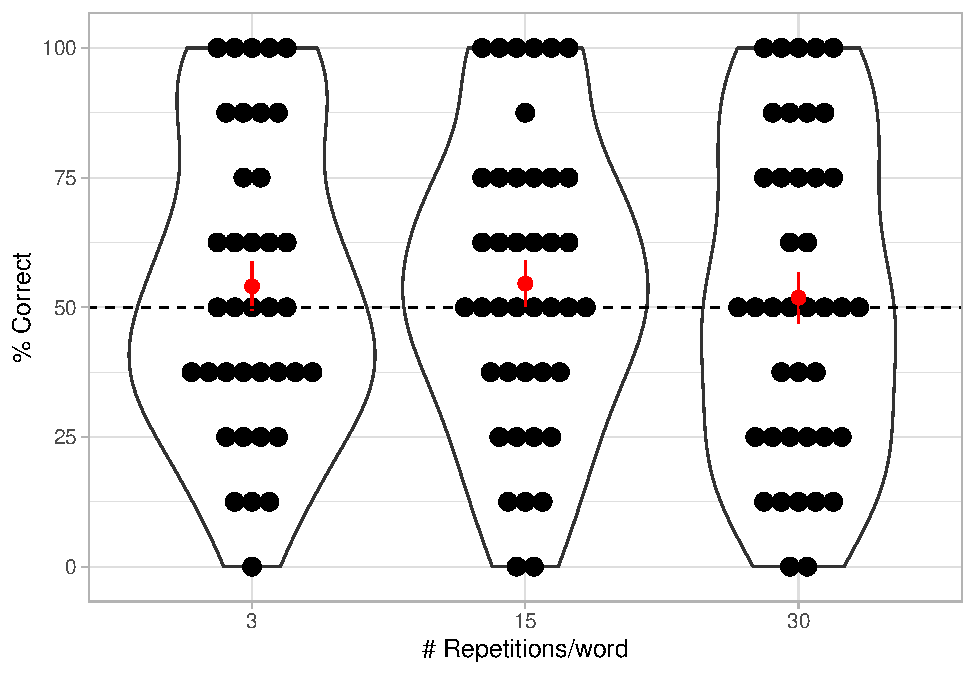
\includegraphics[width=0.8\linewidth]{segmentation_recall_combined_files/figure-latex/bcn-plot-stats-1} 

}

\caption{Results of Pilot Experiment 2. Each dot represents a participants. The central red dot is the sample mean; error bars represent standard errors from the mean. The results show the percentage of correct choices in the recognition test after familiarization with (left) 3, (middle) 15  or (right) 30 repetitions per word.}\label{fig:bcn-plot-stats}
\end{figure}

\begin{table}

\caption{\label{tab:bcn-glmm-print}Performance in Pilot Experiment 2 for different amounts of exposure. The differences were assessed using a generalized linear model for the trial-by-trial data, using participants as a random factor.}
\centering
\begin{tabular}[t]{lrrlrr}
\toprule
Effect & Estimate & Std. Error & CI & t & p\\
\midrule
Language = L2 & 0.337 & 0.493 & -0.629, 1.3 & 0.684 & 0.494\\
\# Word repetitions & 0.017 & 0.018 & -0.018, 0.0513 & 0.942 & 0.346\\
Language = L2 $\times$ \# Word repetitions & -0.042 & 0.025 & -0.0916, 0.00698 & -1.682 & 0.093\\
\bottomrule
\end{tabular}
\end{table}

As shown Table \ref{tab:bcn-glmm-print}, a generalized linear model revealed that performance depended neither on the amount of familiarization nor on the familiarization language. As shown in Figure \ref{fig:bcn-plot-stats}, a Wilcoxon test did not detect any deviation from the chance level of 50\%, neither for all amounts of familiarization combined, \M = 53.5, \SE = 2.71, \p = 0.182, nor for the individual familiarization conditions (3 repetitions per word: \M = 54.1, \SE = 4.81, \p = 0.416; 15 repetitions per word: \M = 54.6, \SE = 4.52, \p = 0.325; 30 repetitions per word: \M = 51.9, \SE = 4.98, \p = 0.63). Following \citet{Glover2004}, the null hypothesis was 4.696 times more likely than the alternative hypothesis after corrections with the Bayesian Information Criterion, and 1.217 more likely after correction with the Akaike Information Criterion.


\end{document}
